
\documentclass[10pt]{report}
\input{/Users/dlr10/papers/Definitions.tex}
\usepackage{geometry}                % See geometry.pdf to learn the layout options. There are lots.
\geometry{letterpaper}                   % ... or a4paper or a5paper or ... 
%\geometry{landscape}                % Activate for for rotated page geometry
%\usepackage[parfill]{parskip}    % Activate to begin paragraphs with an empty line rather than an indent
\usepackage{graphicx}
\usepackage{amssymb}
\usepackage{epstopdf}
\usepackage{color}
\usepackage{appendix}
\usepackage{comment}
\usepackage{latexsym} 
\usepackage{feynmp}
\usepackage{fancyhdr}
\usepackage{array}
\pagestyle{fancy}
%\usepackage{hyperref}
\def \D {{\mathcal D}}
\def\xpp{{x^{\prime\prime}}}
\def\kp{{k^\prime}}
\def\lambdap{{\lambda^\prime}}
\def\kpp{{k^{\prime\prime}}}
\def\bfq{{\bf q}}
\def\xppp{{x^{\prime\prime\prime}}}
\def\kppp{{k^{\prime\prime\prime}}}
\def\Im{{\rm Im}}
\def\H{{\mathcal H}}
\def\pp{{p^{\prime}}}
\def\pdp{{p^{\prime\prime}}}
\def\BFR{{\bf r}}
\def\bfP{{\bf P}}
\def\sdP{{\bf \sigma\cdot P}}
\def\sdp{{\bf \sigma\cdot p}}
\def\bfxp{{\bf x^\prime}}
\def\bfyp{{\bf y^\prime}}
\def\bfkp{{\bf k^\prime}}
\def\bfcr{{\bf R}}
\def\bfP{{\bf P}}
\def\sdP{{\bf \sigma\cdot P}}
\def\sdp{{\bf \sigma\cdot p}}
\def\bfxp{{\bf x^\prime}}
\def\bfkp{{\bf k^\prime}}
\def\ppp{{p^{\prime\prime}}}
\def\rpp{{r^{\prime\prime}}}
\def\bfppp{{\bf p^{\prime\prime}}}
\def\bfpp{{\bf p^{\prime}}}
\def\Nabla{{\bf \nabla}}
\def\hatn{{\bf \hat n}}
\def\hata{{\bf \hat a}}
\def\hatb{{\bf \hat b}}
\def\hatc{{\bf \hat c}}
\def\xp{{x^\prime}}
\def\yp{{y^\prime}}
\DeclareGraphicsRule{.tif}{png}{.png}{`convert #1 `dirname #1`/`basename #1 .tif`.png}
\DeclareGraphicsRule{*}{mps}{*}{}
%\title{Quantum Mechanics II}
%\author{David L. Rubin}
%\date{}                                           % Activate to display a given date or no date
\begin{document}
\begin{flushleft}
July 8, 2016\\
D. Rubin
\vskip 0.1in
{\bf \Large Decoherence of the Muon Distribution in the g-2 Ring}\\
\end{flushleft}

\section*{Introduction}
Muons injected into the g-2 storage ring execute betatron oscillations about the closed orbit. The closed orbit is defined by the magnetic and
electric fields and the beam energy. If the magnetic field is uniform and the electric field linear in the displacement of the muons from the closed 
orbit, and all muons have the same energy, 
then all muons oscillate with the same frequency, independent of amplitude. However, in the g-2 ring, the fields of the electrostatic quadrupoles
have significant nonlinearity. The result is that the betatron frequency will depend on the amplitude of the oscillations. In addition,
the betatron tunes and the revolution frequency are energy dependent. As a result of the amplitude and energy dispendence, the distribution of muons
will oscillate with a spread of frequencies resulting in an eventual decoherence of the betatron motion. The amplitude of the motion of the 
centroid of the distribution, as well as the modulation of the beam width,  will ``damp'' over this decoherence time.
%
%Another contribution to the tune spread is the chromaticity of the guide field. Chromaticity is the energy dependence of the tune. 
%Coherent transverse oscillations of muons in the g-2 storage ring are 'damped' due to amplitude and energy dependence of the betatron tune.
%The amplitude dependence results from the nonlinearity in the field of the quadrupoles. The energy dependence is due to the natural
%chromaticity of the ring. 
%
The particles oscillate coherently at the start of the fill and decohere due to both amplitude and energy dependence of the betatron tunes. 
The amplitude of the modulation of the
width of the injected beam is a measure of the unavoidable mismatch of the twiss parameters at the inflector exit. The amplitude of the oscillations of the beam centroid
will ultimately depend on the quality of the fast kicker pulse. The betatron frequency depends on the amplitude and energy of the particles, and therefore
the oscillations of both width and centroid will decohere after some number of turns.
\section*{Amplitude Dependent Tune}
The multipole expansion of the quadrupole field in the midplane of the ring can be written\cite{NIMesquad}
$$E_x(x) = \sum_{n=1} b_n n\frac{x^{n-1}}{r_0^n}$$
The effective focusing of the quadrupoles is proportional to the field gradient
$$G_x = \partder{E_x}{x}=\sum_{n=1} n(n-1) b_n \frac{x^{n-2}}{r_0^n}$$
In a perfect quadrupole, only $b_2$ is non-zero and $G_x = 2b_n\frac{1}{r_0^2}$, independent of displacement $x$. 
In our imperfect quadrupole,
the gradient depends on the amplitude. We write an effective amplitude dependent gradient 
$$\vev{G_x} = \sum_{n=1} n(n-1) b_n \frac{\vev{x^{n-2}}}{r_0^n}$$
where $\langle x^{n-2}\rangle$ is the average of $x^{n-2}$.
Let's assume that $x =x_0\cos(\omega_{cbo} t)$, a reasonable assumption in our ring where $\beta(s)$ is very nearly constant. Then     
\begin{eqnarray}
\vev{G_x} &=& \sum_{n=1} n(n-1) b_n \frac{x_0^{n-2}}{r_0^n}\vev{\cos^{n-2}(\omega t)}\label{gradient}\\
%\vev{G_x} &=& \sum_{n=1}^N 2m(2m-1) b_{2m} \frac{x_0^{2m-2}}{r_0^{2m}}\vev{\cos^{2n-2}(\omega t)}\\
\end{eqnarray}
and the contribution from all odd $n$ is zero.
The effective gradient is then given by
$${G_A(x_0)} = \sum_{n=1}^N n(n-1) b_{n} \frac{x_0^{n-2}}{r_0^{n}}c_{n-2}$$
where $c_{n-2} = \vev{\cos^{n-2}\omega t}$ and $x_0$ is the amplitude.
The multipoles for the g-2 ring quadrupoles are summarized in Table~\ref{quadparams}.
\begin{table}[b]
\caption{}
\begin{center}
\begin{tabular}{|l|l|l|c|}
\hline
Multipole (n) & Value [${\rm V/m^n}$]&$c_{n-2}$& $\Delta {\rm Q_x/m^n}$\\ \hline
2&26331.0 &0& 0 \\
4&43.06 & $1/2$&$1.26\times 10^{8}$\\
6& -59.90&${3}/{8}$&$-1.08\times 10^{11}$\\
8& -7.18&${5}/{16}$&$-8.96\times 10^{12}$\\
10& -510.63&${35}/{128}$&$-4.22\times 10^{17}$\\
12& -8.48&${63}/{256}$&$-4.44\times 10^{18}$\\
14& 68.25&$231/1024$&$2.19\times 10^{22}$\\
\hline
\end{tabular}
\end{center}
\label{quadparams}
\end{table}

The tune shift due to an electric field gradient error $G(s)$ is $$\Delta Q = \frac{1}{4\pi}\oint\beta q\frac{E_x(s)}{dx}\frac{1}{pv}ds$$
where $q$, $p$, and $v$ are the muon charge, momentum and velocity respectively. Using $R=mv/qB$ 
the tune shift becomes $$\Delta Q = \frac{1}{4\pi}\oint\beta \frac{E_x(s)}{dx}\frac{1}{RBv}ds$$
Then the amplitude dependent tune shift is 
$$\Delta Q(x,s) = \frac{1}{4\pi}\oint \beta \frac{ G_A(x,s)}{RBv} ds$$
The gradient $G_A(s)$ is given by Equation~\ref{gradient} in the quads and is zero everywhere else.
Since the quads extend over a length
$L = 4(2\pi\frac{39}{360}(7.112))$ we write
\begin{equation}
\Delta Q(x,s) = \frac{1}{4\pi} \beta \frac{ G_A(x,s)}{RBv} L\label{eq:analytic_tuneshift}
\end{equation}
The contribution to the horizontal tune shift from each of the multipoles is shown in Table~\ref{quadparams} and in Figure \ref{mp_tuneshift}.
%If $b(1)$ is chosen for a field index of 0.141, the values in the table follow
%        Er     = Er     + (n/r0) * (r/r0)**(n-1) * ( QMC(0,1,n)*cos(n*theta) + QMC(0,2,n)*sin(n*theta) )
%  REAL(RP) :: r0 = 0.045
\begin{figure}[htbp] %  figure placement: here, top, bottom, or page
   \centering
   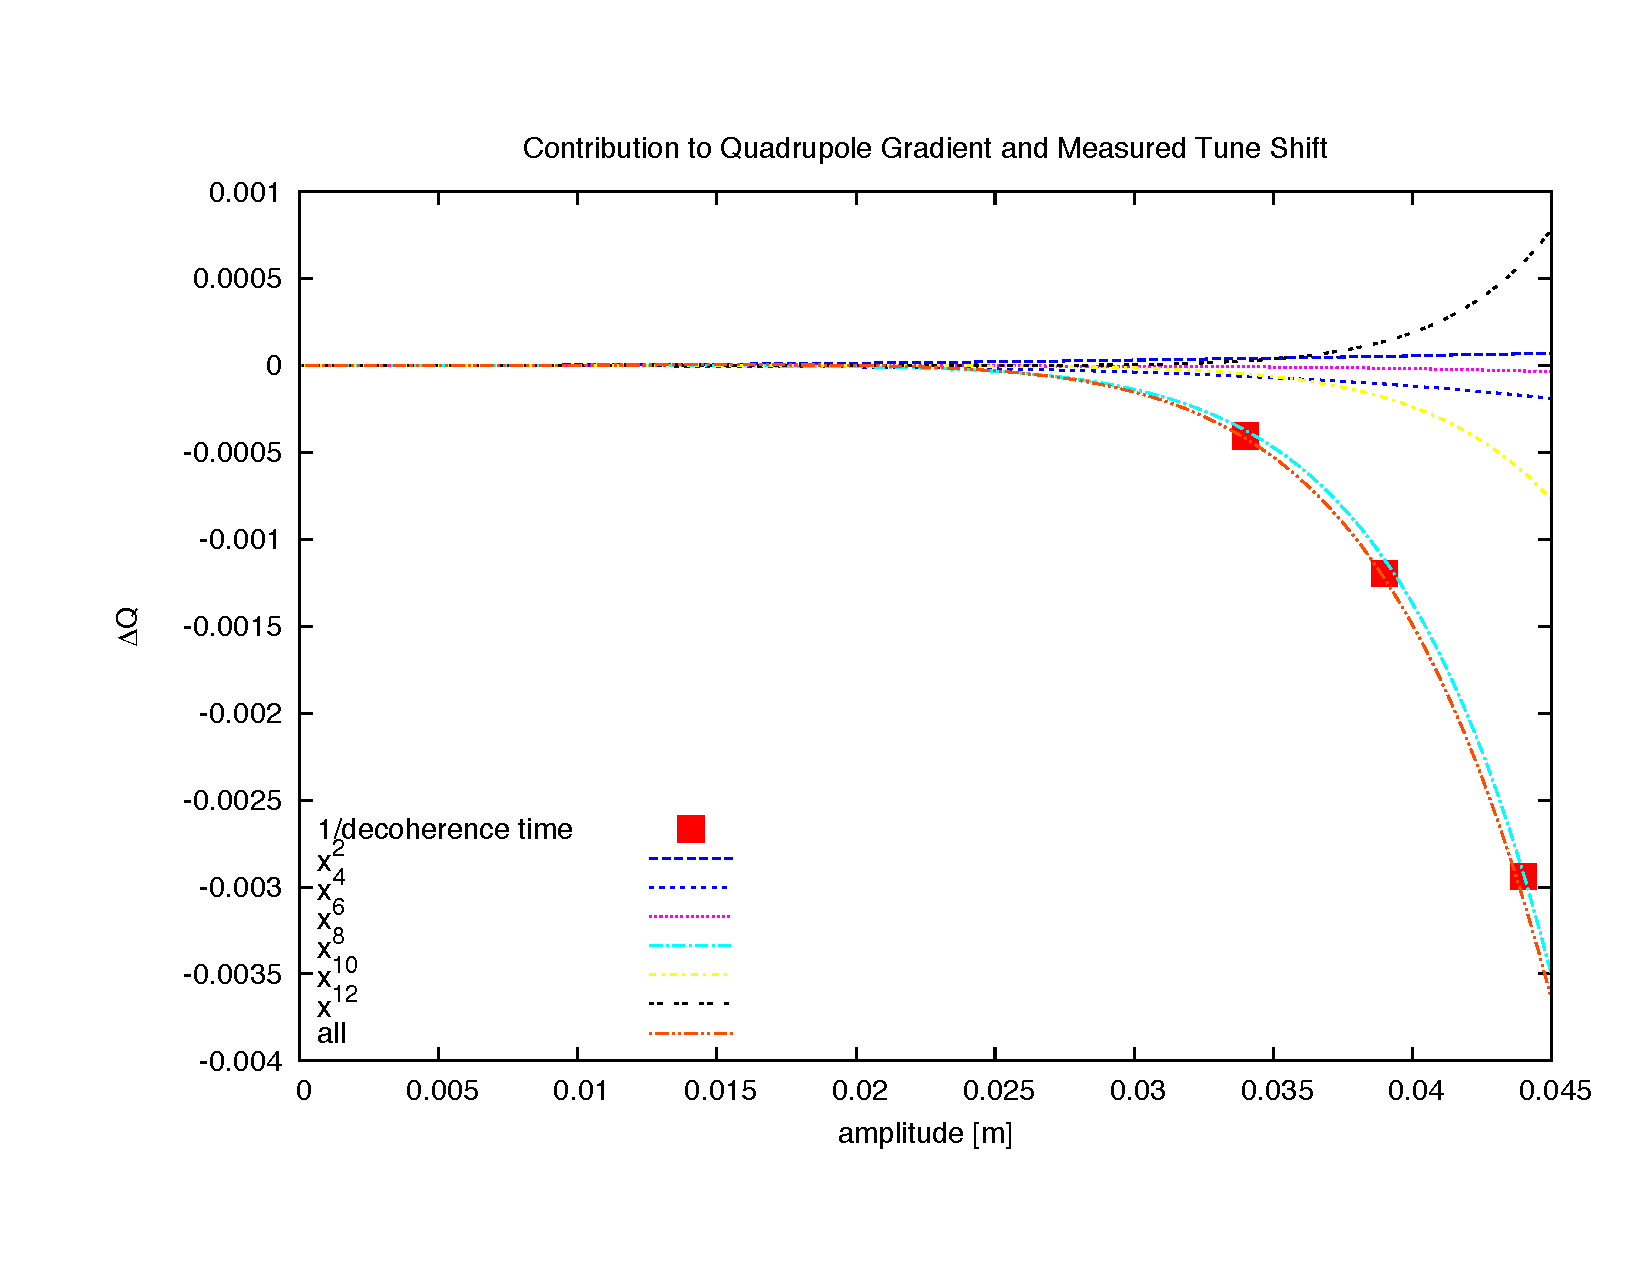
\includegraphics[trim = 10mm 0mm 0mm 40mm, clip=.false.,width=6.in]{/Users/dlr10/lepp/g-2/beamdynamics/damping_cbo/tuneshift.pdf} 
   \caption{Tuneshift as a function of betatron amplitude (Equation~\ref{eq:analytic_tuneshift} for each of the quadrupole multipoles (lines) and as computed by tracking (squares) for
three different amplitudes.
 \label{mp_tuneshift}}
\end{figure}
\section*{Tune spread and decoherence}
The analytic calculation of the amplitude dependent tune shifts can be checked in simulation. 
Suppose the tunes for two different muons are split by $\Delta Q$.
The sum of the displacements of the two muons at $Q$ and $Q +\Delta Q$ on turn $n$ is
\begin{eqnarray*}
x(n)&=&A\sin (2\pi Q n) + A\sin(2\pi (Q+\Delta Q)n)
\end{eqnarray*}
where $\bar Q$ is the average of the tunes. Note that if $n\Delta Q = \frac{1}{2}$ then the particles are $180^\circ$ out of phase. The decoherence time (in units of turns) is
$T = \frac{1}{2\Delta Q}$.
Track two particles with initial amplitudes of about 4 cm. For one of the particles, turn off all multipoles $n>2$ so that the guide field is linear and tune is independent
of amplitude. For the other, restore all quad multipoles. The oscillation of the two particles is shown in Figure~\ref{overlay}


\begin{figure}[htbp] %  figure placement: here, top, bottom, or page
\begin{minipage}[t]{0.48\textwidth}
   \centering
   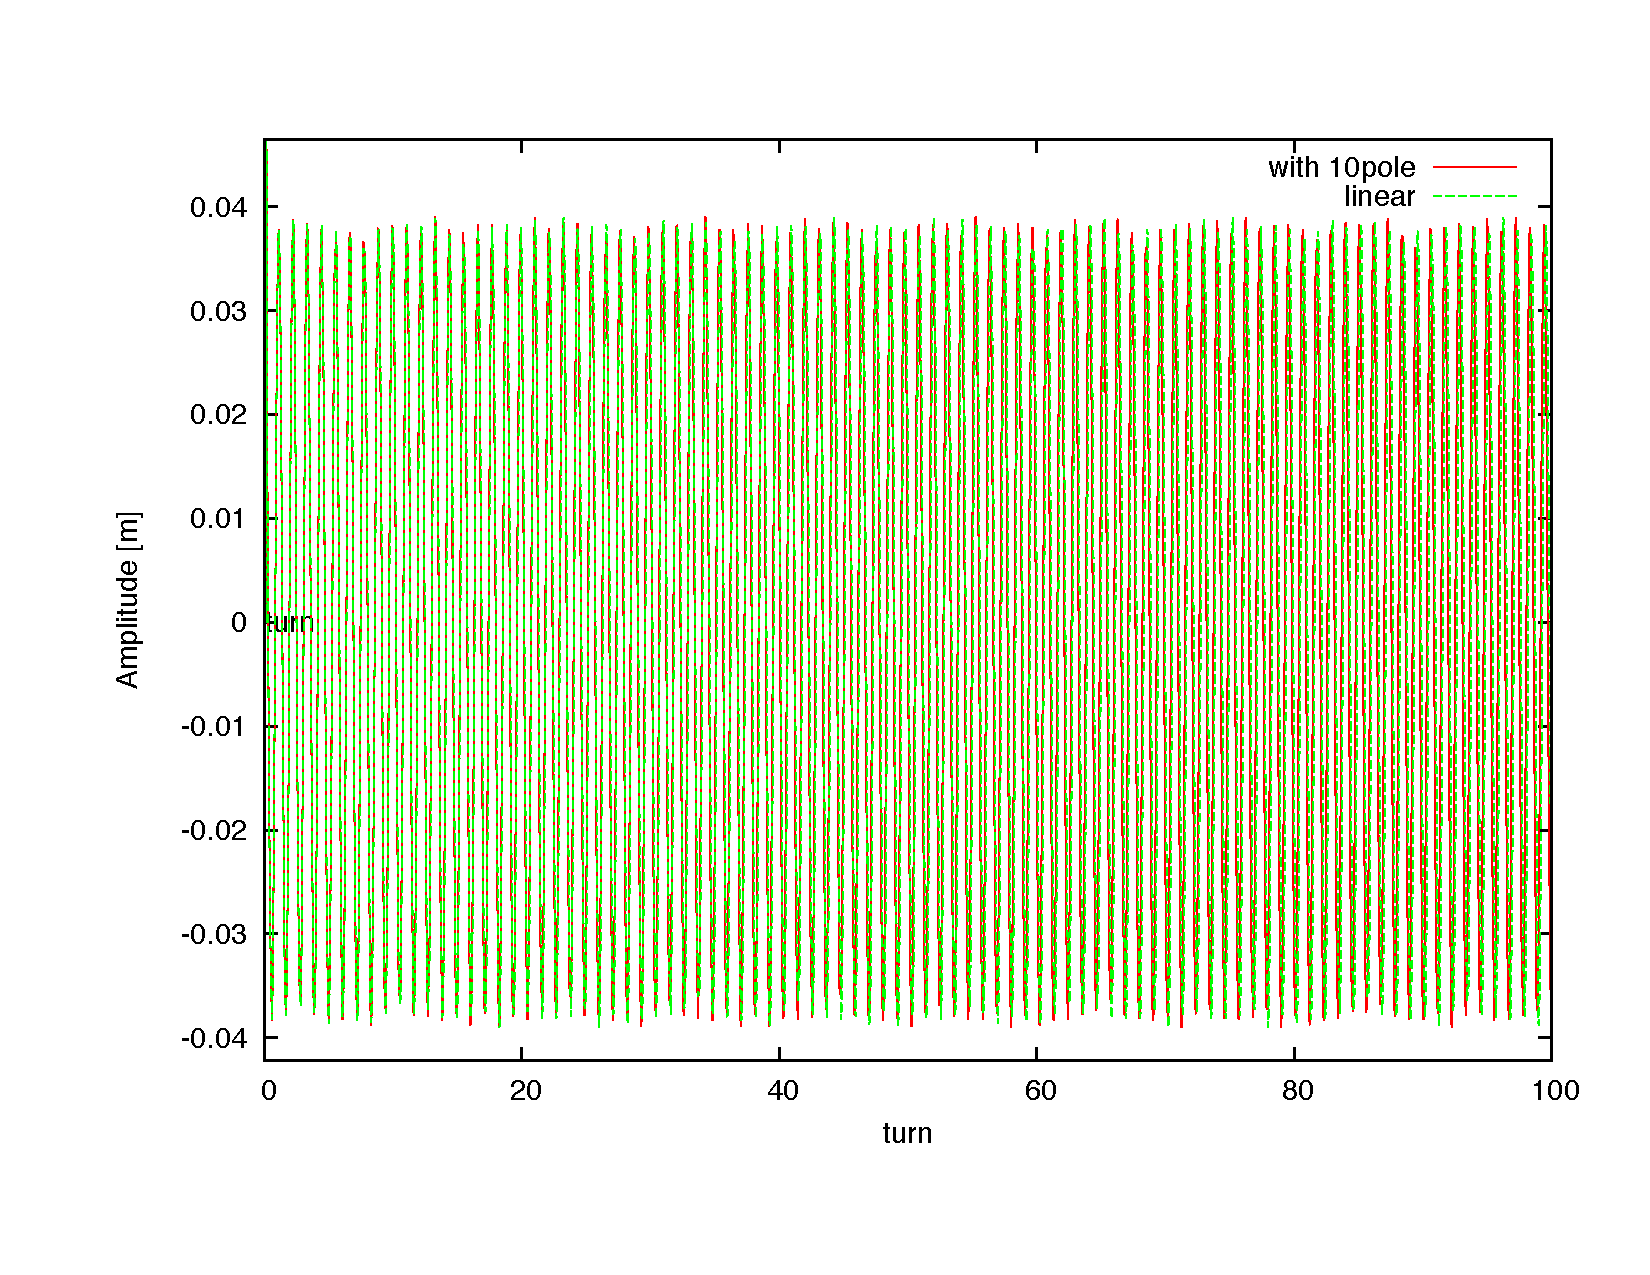
\includegraphics[trim = 0mm 0mm 0mm 0mm, clip=.false.,width=3.in]{/Users/dlr10/lepp/g-2/beamdynamics/damping_cbo/tune_overlay_linear_10_4cm.pdf} 
   \caption{Horizontal displacement vs turn number. The green line is with purely linear quadrupole fields, (no multipoles). The red line
is with all quad multipoles included. The amplitude of the oscillation is about 3.9 cm. \label{overlay}}
 \end{minipage}
\hfill
\begin{minipage}[t]{0.48\textwidth}
\centering
   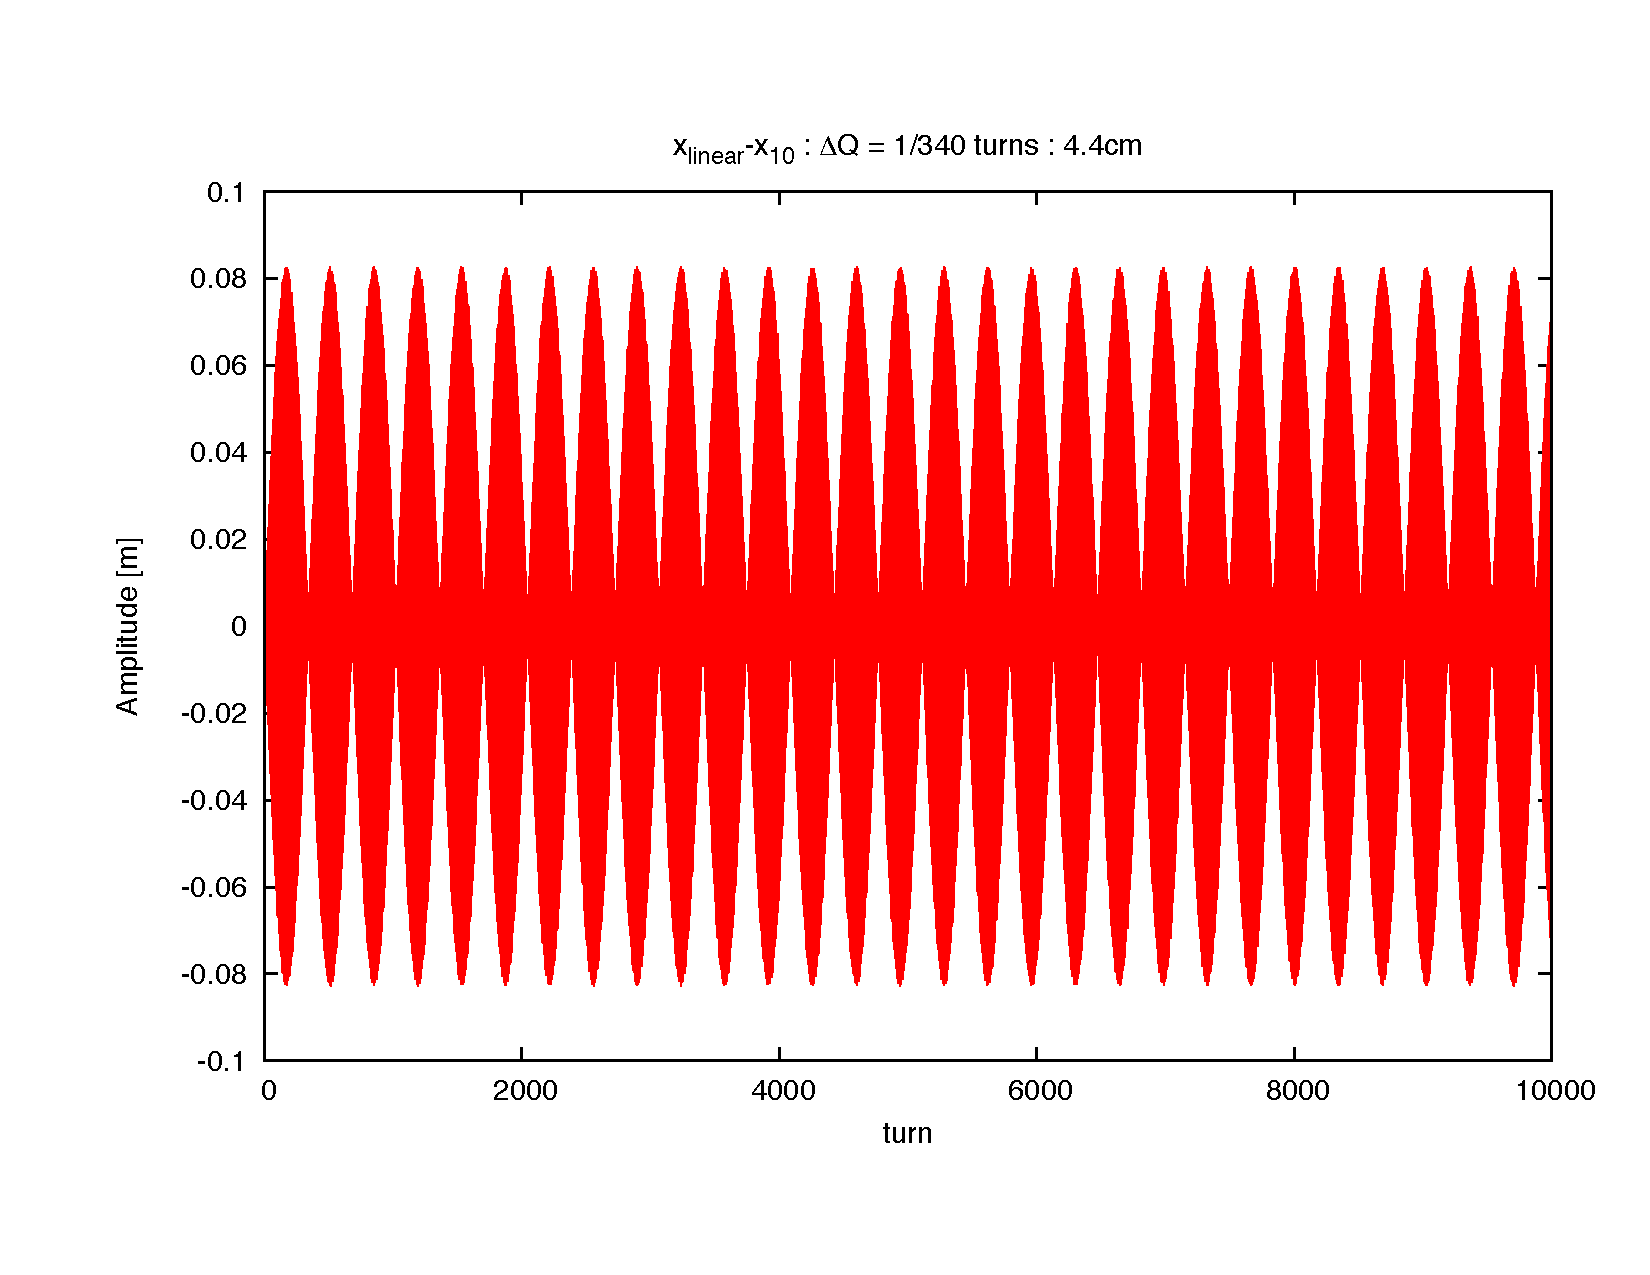
\includegraphics[trim = 0mm 0mm 0mm 0mm, clip=.false.,width=3.in]{/Users/dlr10/lepp/g-2/beamdynamics/damping_cbo/tune_difference_linear-allpole_44mm.pdf} 
\caption{Sum of displacements with and without quad multipoles when the oscillation amplitude is 4.4 cm. The beat frequency corresponds to the tune difference.
   \label{difference44}}
\end{minipage}
\end{figure}

The sum of the displacements of the two particles is
\begin{eqnarray*}
x_1(n)+x_2(n) &=& A\left(\sin(2\pi (\bar Q+\Delta Q/2) n)+\sin(2\pi(\bar Q-\Delta Q/2)n)\right)\\
&=& A\left(\sin(2\pi (\bar Q+\Delta Q/2) n)+\sin(2\pi(\bar Q-\Delta Q/2)n)\right)\\
&=& 2A\sin(2\pi \bar Q n)\cos(2\pi\Delta Q n)
\end{eqnarray*}
and shown in Figure~\ref{difference44}. The signal at $\bar Q$ is modulated at the tune difference.
From Figure~\ref{difference44}, we see that $\Delta Q (44{\rm mm})$ is 1/340 ${\rm turns}$.

We use the same strategy to determine the tune shift for amplitudes of 39 mm and 34 mm. The turn by turn sum
of trajectories with and without quad nonlinearities are shown in Figures~\ref{difference39} and~\ref{difference34} respectively.
The amplitude dependence of the tune shift as determined by tracking is plotted in Figure~\ref{mp_tuneshift} along with
the analytic calculation. Analytic and numerical results are in reasonable agreement. 
%
%All multipoles vs none
%Amplitude       Delta Turns
%0.039               838
%0.044               340
%0.034               2470

\begin{figure}[htbp] %  figure placement: here, top, bottom, or page
\begin{minipage}[t]{0.48\textwidth}
   \centering
   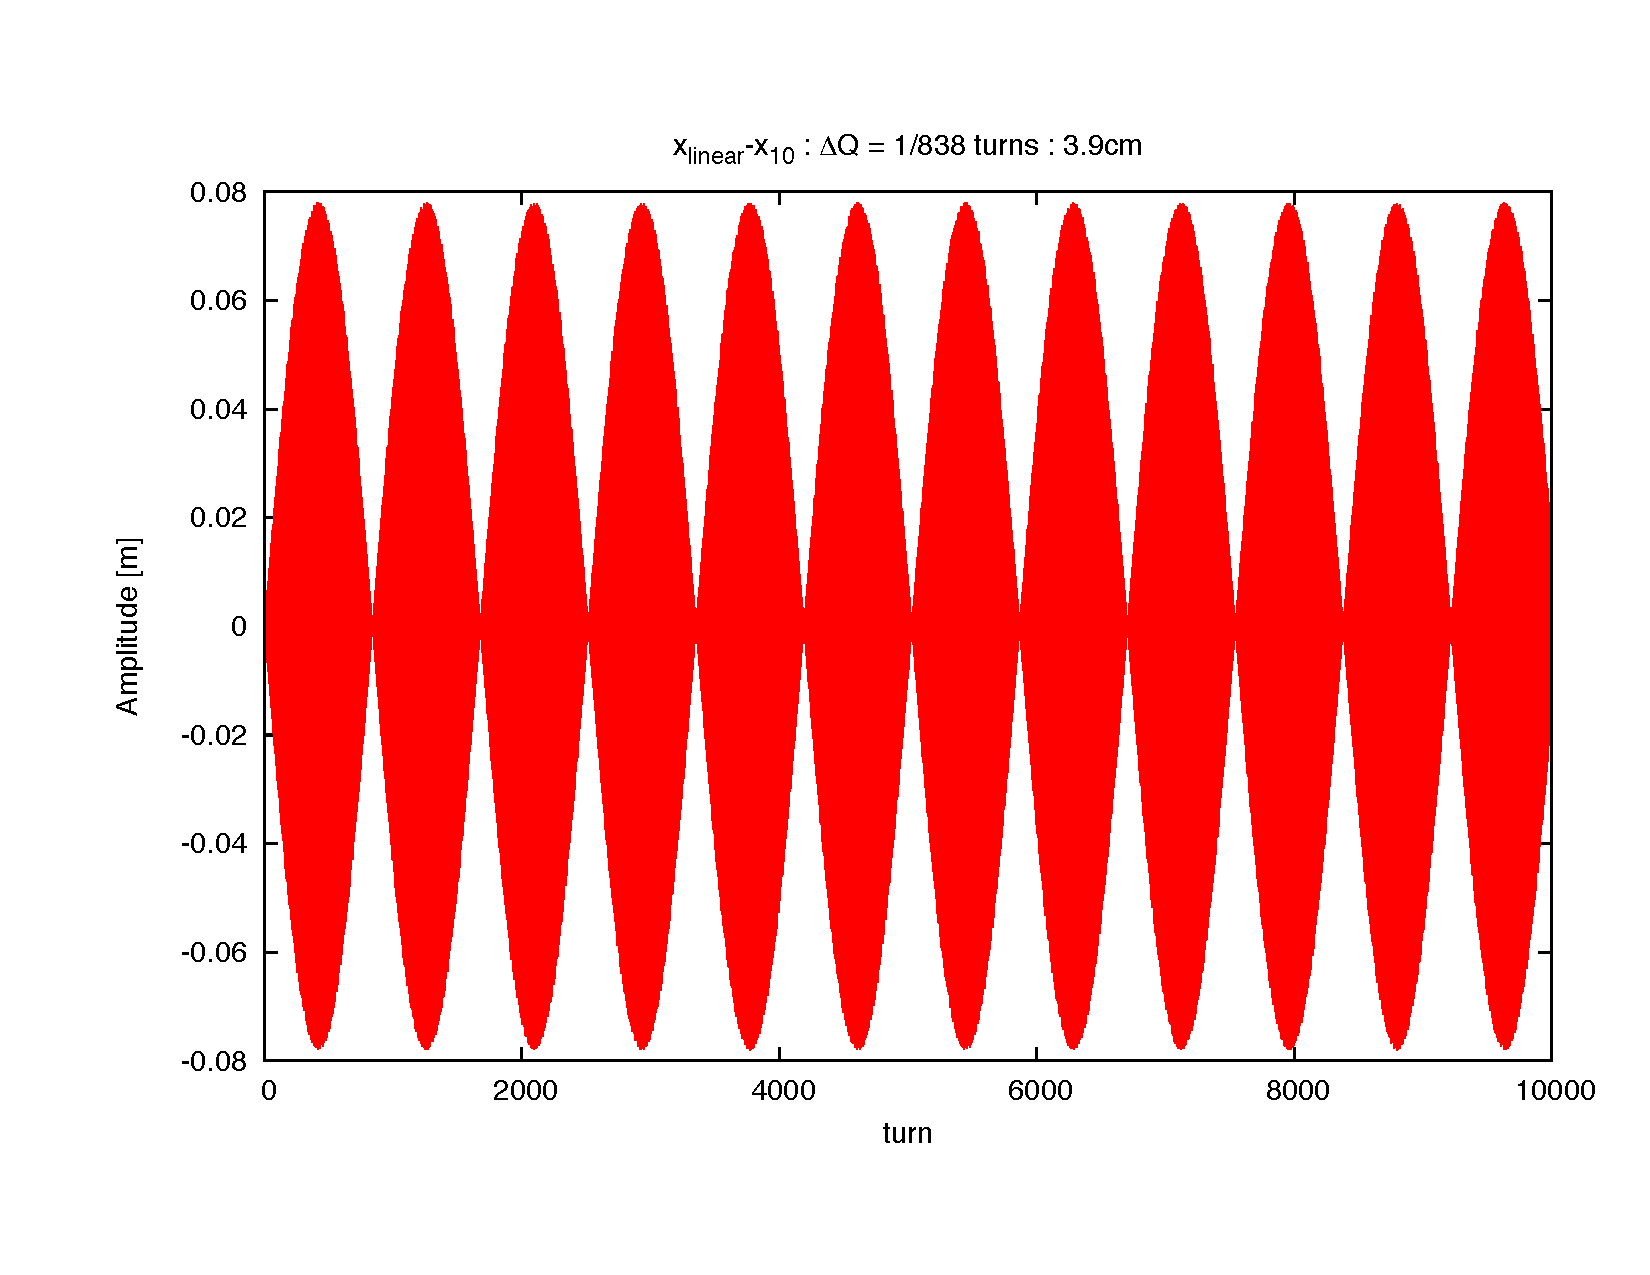
\includegraphics[trim = 0mm 0mm 0mm 0mm, clip=.false.,width=3.in]{/Users/dlr10/lepp/g-2/beamdynamics/damping_cbo/tune_difference_linear_all_39mm.pdf} 
   \caption{Sum of displacements with and without quad multipoles (nonlinearities) when the oscillation amplitude is 3.9 cm as in 
Figure~\ref{overlay}. $\Delta Q$ = 1/838 turns. \label{difference39}}
 \end{minipage}
\hfill
\begin{minipage}[t]{0.48\textwidth}
\centering
   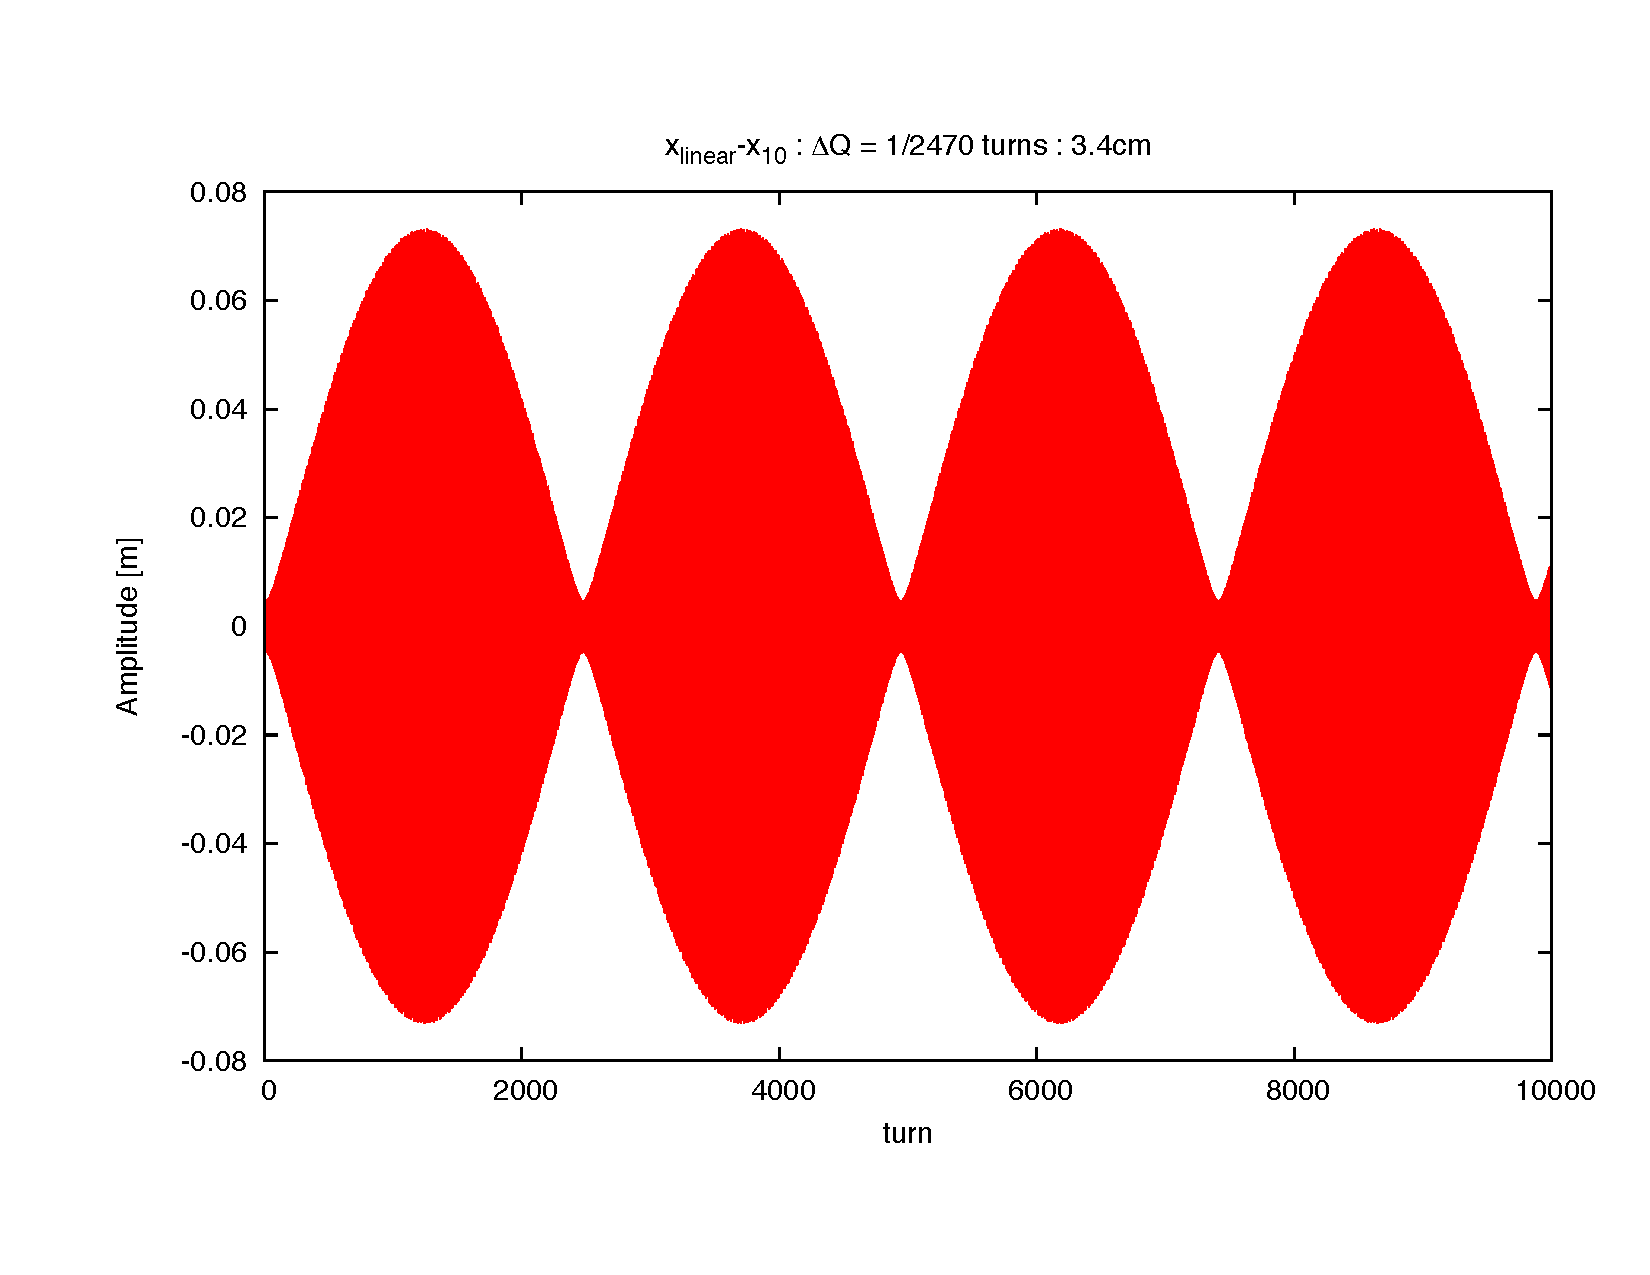
\includegraphics[trim = 0mm 0mm 0mm 0mm, clip=.false.,width=3.in]{/Users/dlr10/lepp/g-2/beamdynamics/damping_cbo/tune_difference_linear_all_34mm.pdf} 
\caption{Sum of displacements with and without quad multipoles when the oscillation amplitude is 3.4 cm. $\Delta Q = 1/2470$ turns. 
   \label{difference34}}
\end{minipage}
\end{figure}

\section*{Decoherence in a distribution}
Consider a distribution of 1000 muons with 95\% horizontal and vertical emittance of 40mm-mrad. Suppose the residual coherent 
betatron oscillation amplitudes are 10mm horizontally and about 1mm vertically. Due to the beta mismatch the width of the distribution
varies from 6 to 13 mm and the height from 8 to 16mm. As described above the effect of the quadrupole nonlinearity
is to introduce an amplitude dependent tuneshift.  Vertical and horizontal centroid and width over the first 2000 turns
is shown in Figure~\ref{distribution_nomp}. Here the quad nonlinearity is turned off so there is no decoherence.
 

\begin{figure}[htbp] %  figure placement: here, top, bottom, or page
   \centering
   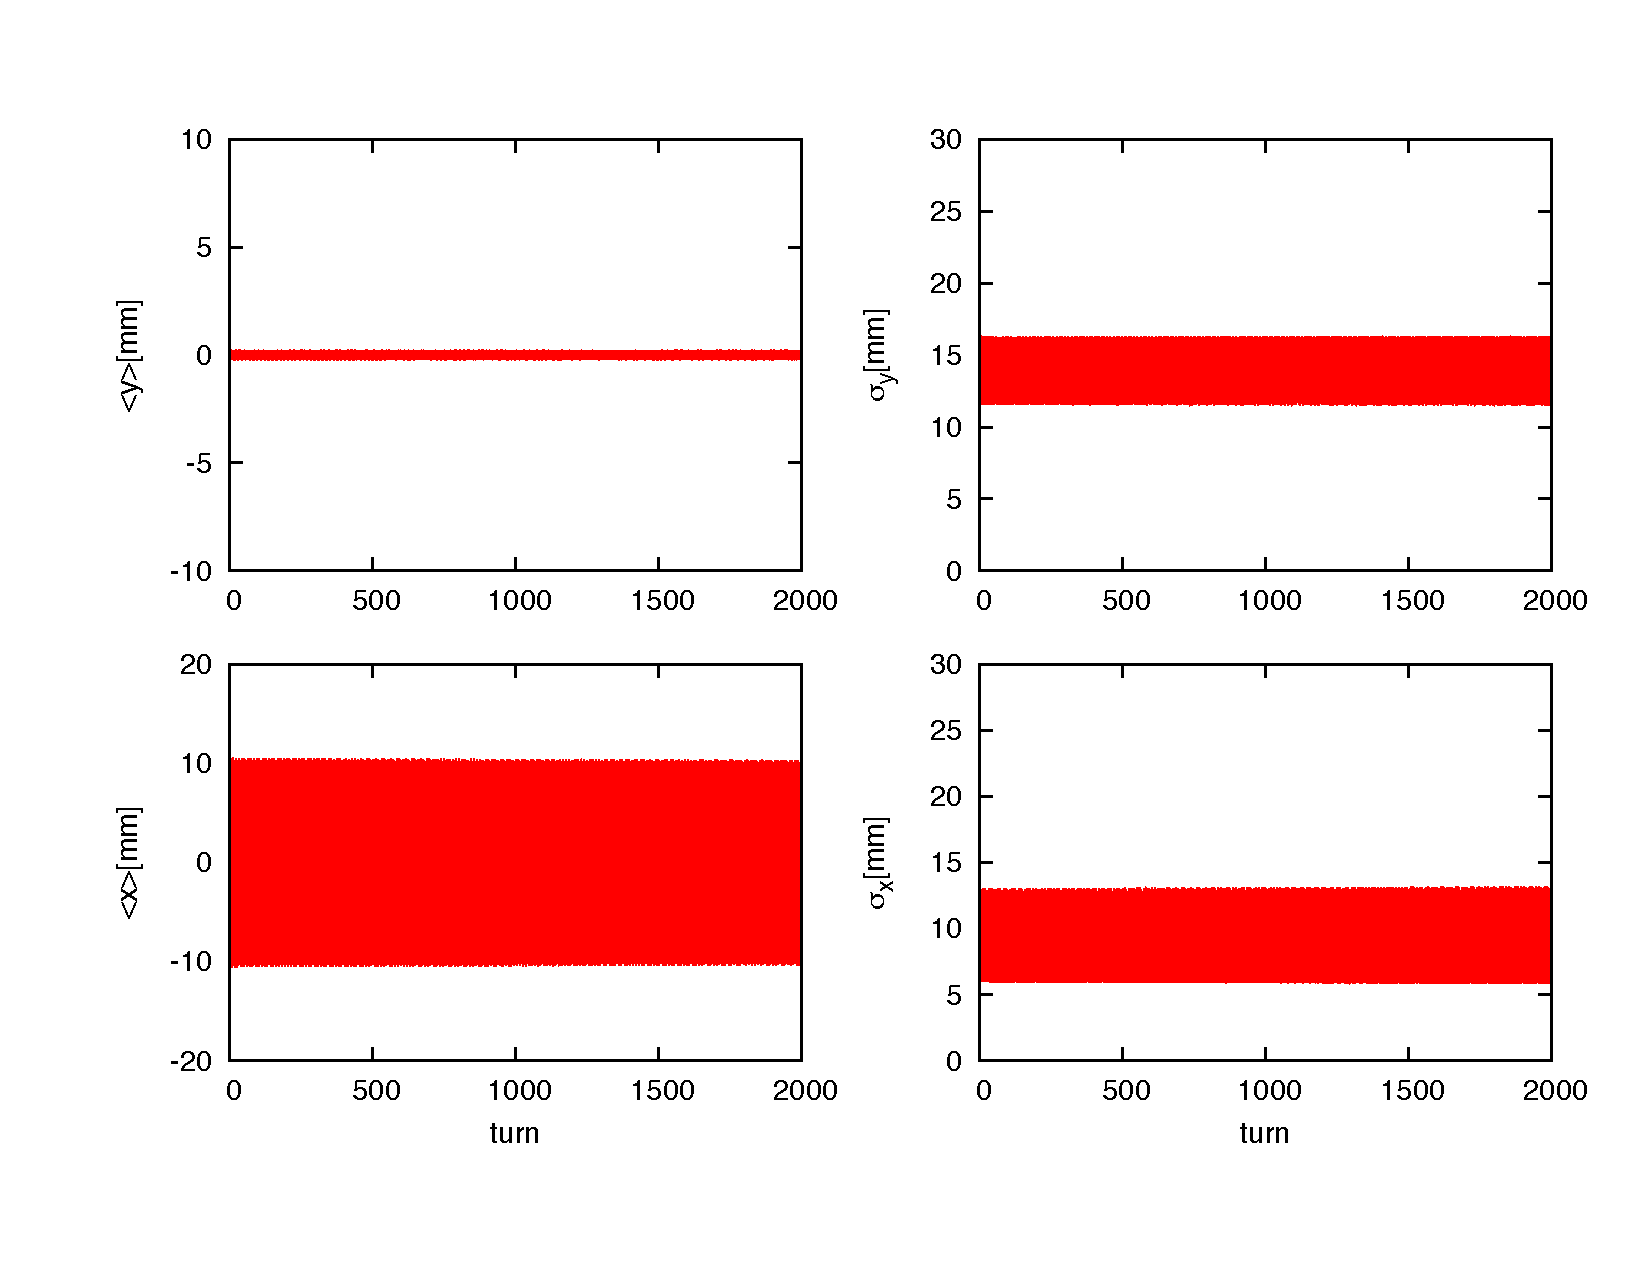
\includegraphics[trim = 40mm 0mm 0mm 0mm, clip=.false.,width=7.in]{/Users/dlr10/lepp/g-2/beamdynamics/damping_cbo/sigma_xy_qm01_deltae0} 
   \caption{With no quad nonlinearities, average horizontal (bottom-left) and vertical (top-left) centroid motion versus turn.
Horizontal and vertical beam width versus turn is at right. \label{distribution_nomp}}
\end{figure}
The decoherence is evident in the evolution of the distribution with quad nonlinearity restored as shown in Figure~\ref{dist_mp}. 
The amplitude of the coherent horizontal betatron oscillation shrinks by a factor of two
in 2000 turns. The variation in the width and height of the distribution also ``damps'' on a time
scale of 1000 turns. Note that the particles remain bunched, as they all have the same energy.


\begin{figure}[htbp] %  figure placement: here, top, bottom, or page
   \centering
   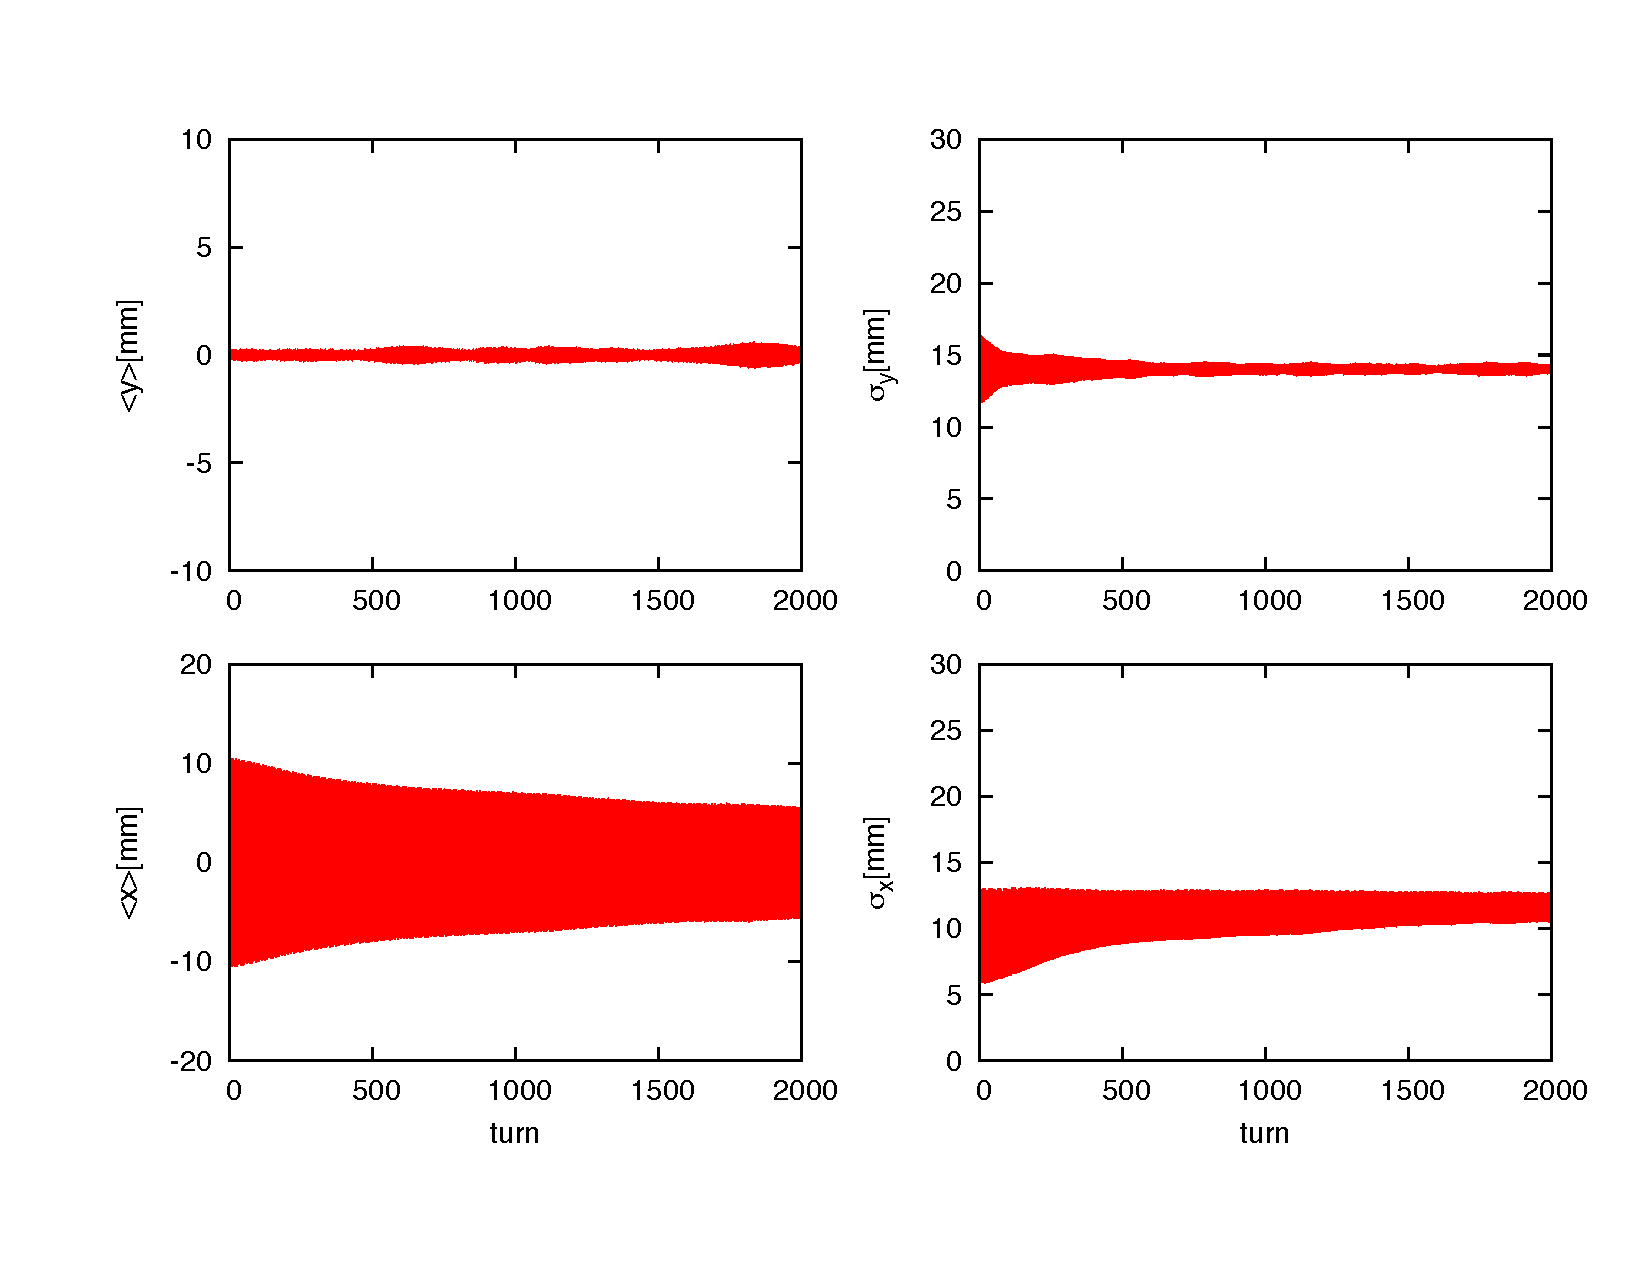
\includegraphics[trim = 40mm 0mm 0mm 0mm, clip=.false.,width=7.in]{/Users/dlr10/lepp/g-2/beamdynamics/damping_cbo/sigma_xy_qm_all_deltae0_10mm} 
   \caption{ With quad linearities, average horizontal (bottom-left) and vertical (top-left) centroid motion versus turn.
Horizontal and vertical beam width versus turn is at right. Decoherence of centroid motion and modulation of beam width is evident.\label{dist_mp}}
\end{figure}
\newpage
\section*{Momentum spread}
The energy dependence of the betatron tunes and the revolution frequency, contribute to the decoherence of betatron motion due to the finite energy spread in the beam.
In a cyclotron with electrostatic focusing
distributed uniformly around the ring,
the tune depends on the focusing index $n$. 
\begin{eqnarray*}
Q_x &=& \sqrt{1-n}\\
Q_y &=& \sqrt{n}
\end{eqnarray*}
where $$n =\left(\frac{r}{v_s B}\right)\partder{E_r}{r}$$
where $r$ is the radius of curvature of the on muon with momentum $p$ in magnetic field $B$ and $v_s$ is the azimuthal
velocity, that is $r = \frac{\gamma m v_s}{q B} = \frac{p}{qB}$.
The dependence of betatron tune on energy, (chromaticity) follows from
$$n(\delta) = \frac{p(1+\delta)}{qv_s B^2}$$ so
that
\begin{eqnarray*}
\partder{Q_x}{\delta} &=&-\frac{1}{2}\frac{1}{ \sqrt{1-n}}\partder{n}{p} = -\frac{n}{2\sqrt{1-n}} =-0.103\\
\partder{Q_y}{\delta} &=& \frac{n}{2\sqrt{n}} = 0.215 
\end{eqnarray*}
for $n=0.185$.
Note that the horizontal tune decreases with energy while the vertical tune increases with energy.
In the g-2 ring the quadrupoles extend over $156^{\circ}$ of the circumference.
A more careful calculation that accounts for the nonuniformity of the $\beta$-functions gives
\begin{eqnarray*}
Q^\prime_x&=& -0.14\\
Q^\prime_y&=& 0.31
\end{eqnarray*}
Suppose that all of the particles in the initial distribution all appear in the ring at the
same point in space and time but with a spread in energy. The particles will execute betatron
oscillations with a frequency that depends on the energy, namely $Q_x(\Delta) = Q^\prime_x\Delta$
and $Q_y(\Delta) = Q_y^\prime \Delta$, where $\Delta$ is the fractional energy offset. 
The particles will circulate with cyclotron frequencies
$\frac{1}{\omega(\Delta)} = \frac{1+\Delta}{\omega_0}$.
The betatron frequency
\begin{eqnarray*}
f &=& Q\omega \ {\rm becomes} \\
f &\rightarrow& (Q+Q^\prime\Delta)\frac{\omega_0}{1+\Delta}\\  
%&\sim& (Q+Q^\prime\delta)\omega_0(1-\delta)\\
%&\sim& Q\omega_0 +\delta(Q^\prime-Q)\omega_0 
\end{eqnarray*}
%The average over all momenta is
%\begin{eqnarray*}
%\langle x \rangle &=& x_0\left(\cos(Q\omega_0 t)\langle\cos(Q^\prime-Q)\delta\omega_0 t\rangle
%-\sin Q\omega_0 t \langle \sin(Q^\prime-Q)\delta\omega_0 t\rangle\right)\\
% &=& x_0\left(\cos(Q\omega_0 t)\sum_{\delta_i}\cos(Q^\prime-Q)\delta_i\omega_0 t
%-\sin Q\omega_0 t\sum_{\delta_i} \sin(Q^\prime-Q)\delta\omega_0 t\right)\\
%\end{eqnarray*}
%For any energy distribution symmetric about zero, the ``$\sin$'' term vanishes. 

%\subsection{Flat energy distribution}
%If the distribution
%is flat over the range $\pm\delta_0$ then
%\begin{eqnarray}
%\sum_{\delta}\cos(Q^\prime-Q)\delta_i\omega_0 t &\rightarrow& \frac{1}{2\delta_0}\int_{-\delta_0}^{\delta_0}
%\cos (Q^\prime -Q)\delta_i\omega_0 t d\delta\nonumber\\ 
%&=& \frac{1}{\xi}
%\left(\sin(\xi \delta_0)+\sin(\xi\delta_0)\right)\nonumber\\
%&=& 2\frac{\sin\xi \delta_0}{2\delta_0\xi}\label{energy_width}
%\end{eqnarray}
%where $\xi = (Q^\prime-Q)\omega_0 t$. According to~\ref{energy_width},
%the average position of all of the particles is zero when
%\begin{eqnarray*}
%\xi\delta_0 &=& \pi \\
%\rightarrow t&=& \frac{\pi}{(Q^\prime-Q)\omega_0\delta_0}
%\end{eqnarray*}
%Let's compute the horizontal and vertical decoherence times in units of the revolution period.
%\begin{eqnarray*}
%N_x &=& \frac{\omega_0 t}{2\pi} = \frac{\pi}{(-0.14 - 0.908)2\pi(0.0012)}=909\\
%N_y &=& \frac{1}{2(0.31-0.43)0.0012} = 3571
%\end{eqnarray*}

%\subsection{Gaussian energy distribution}
%If the distribution of energies is Gaussian with width $\delta_0$ then
%$$x(t) = \delta\eta\cos\left((Q+(Q^\prime-Q)\delta)\omega_0 t\right)$$
%\begin{eqnarray*}
%\sum_{\delta}\cos(Q^\prime-Q)\delta_0\omega t&\rightarrow& \frac{1}{\delta_0\sqrt{2\pi}}\int_{-\infty}^\infty\cos\xi\delta {e^{-\frac{1}{2}\frac{\delta^2}{\delta_0^2}}}d\delta\\
%&=& \frac{1}{2\delta_0\sqrt{2\pi}}
%\int_{-\infty}^\infty\left(e^{i\xi\delta}+e^{-i\xi\delta}\right) 
%e^{-\frac{1}{2}\frac{\delta^2}{\delta_0^2}}d\delta\\
%&=& \frac{2}{2\delta_0\sqrt{2\pi}}e^{-\frac{1}{2}\xi^2\delta_0^2}(\sqrt{2\pi}\delta_0)\\
%&=& e^{-\frac{1}{2}\xi^2\delta_0^2}
%\end{eqnarray*}

\section*{Fast Rotation}
Imagine that the initial distribution has zero emittance, zero energy spread and zero bunch length.
The particles share a common revolution period $T$ and the time dependence of the intensity signal
at a fixed point in the ring (a fiber harp for example), is $$I(t) = \delta(t-nT)$$
where $n$ is any non negative integer. A particle with energy offset $\Delta$ will have revolution period $T(1+\Delta)$, so that
$$I(t,\Delta) = \delta(t-nT(1+\Delta))$$
The signal in the fiber harps is given by
\begin{eqnarray*}
S(t) &=& \sum_{n=0}^\infty \int \rho(\Delta) \delta(t-nT(1+\Delta)) d\Delta
\end{eqnarray*}
where $\rho(\Delta)$ is the distribution of momenta offsets. If the energy distribution is Gaussian with width $\Delta_0$, then
\begin{eqnarray}
S(t)&=& \sum_{n=0}^\infty \int \frac{e^{-\Delta^2/(2\Delta_0^2)}}{\sqrt{2\pi}\Delta_0} \delta(t-nT(1+\Delta)) d\Delta\nonumber\\
&=& \sum_{n=0}^\infty \int \frac{e^{-\Delta^2/(2\Delta_0^2)}}{\sqrt{2\pi}\Delta_0} \frac{\delta(\Delta-(\frac{t}{nT}-1)}{nT} d\Delta\nonumber\\
&=& \sum_{n=0}^\infty\frac{e^{-(\frac{t}{nT}-1)^2/(2\Delta_0^2)}}{\sqrt{2\pi}\Delta_0 nT}\label{eq:fr}
\end{eqnarray}
For energy spread $\Delta_0= 0.0012$, which is just about the acceptance of the g-2 ring, $S(t)$ from Equation~\ref{eq:fr} is shown
in Figures~\ref{fig:fastrotation_0-20},~\ref{fig:fastrotation_5-10}, and~\ref{fig:fastrotation_15-20}. 
Figures~\ref{fig:fastrotation_5-10}, and~\ref{fig:fastrotation_15-20} are the same data as~\ref{fig:fastrotation_0-20} on expanded horizontal scale.
The intensity asymptotically approaches that of the average stored current $\langle I\rangle = eN_\mu /T$.
(Note that there is no muon decay in Equation~\ref{eq:fr} or the accompanying plots).

\begin{figure}[htbp] %  figure placement: here, top, bottom, or page
%\begin{minipage}[t]{0.8\textwidth}
   \centering
   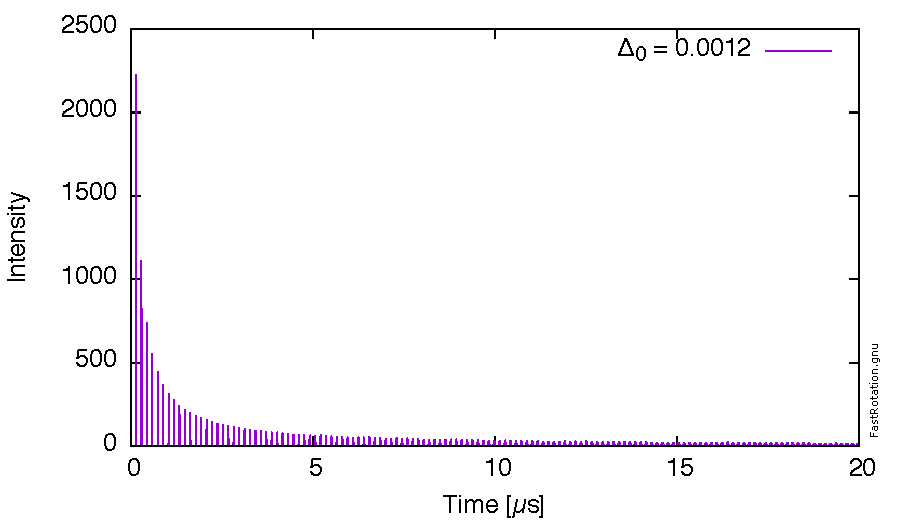
\includegraphics[trim = 0mm 0mm 0mm 0mm, clip=.false.,width=6.in]{/Users/dlr10/lepp/g-2/beamdynamics/damping_cbo/FastRotation_0-20.pdf} 
   \caption{Fast rotation signal 0-20$\mu$s. \label{fig:fastrotation_0-20}}
% \end{minipage}
\end{figure}
\begin{figure}[htbp] %  figure placement: here, top, bottom, or page
\begin{minipage}[t]{0.48\textwidth}
   \centering
   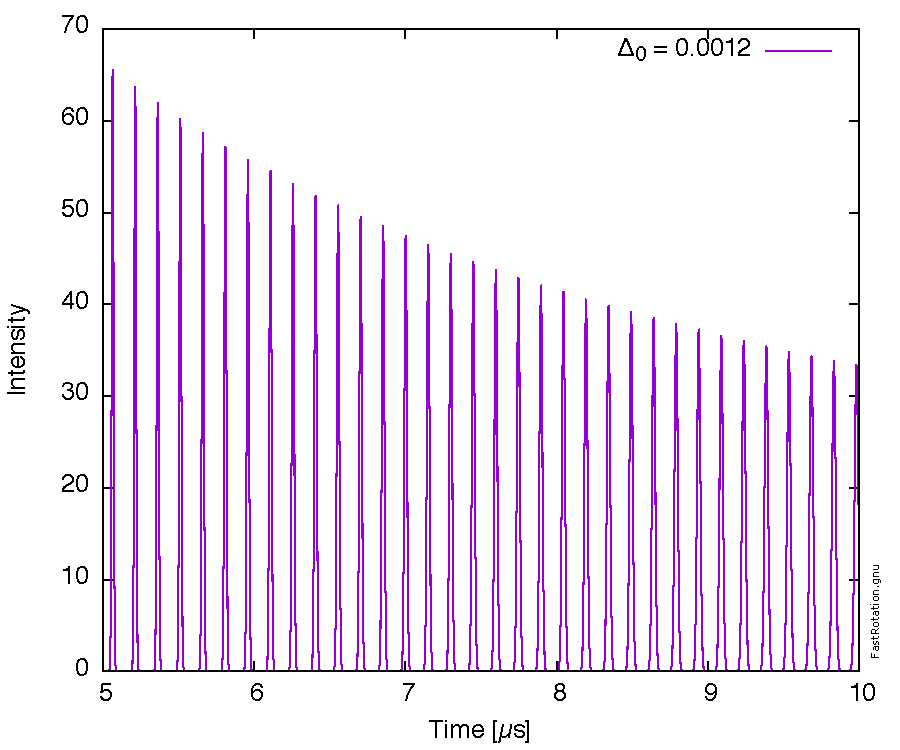
\includegraphics[trim = 0mm 0mm 0mm 0mm, clip=.false.,width=3.in]{/Users/dlr10/lepp/g-2/beamdynamics/damping_cbo/FastRotation_5-10.pdf} 
   \caption{Fast rotation signale from 5$\mu$s to 10$\mu$s \label{fig:fastrotation_5-10}}
 \end{minipage}
\hfill
\begin{minipage}[t]{0.48\textwidth}
\centering
   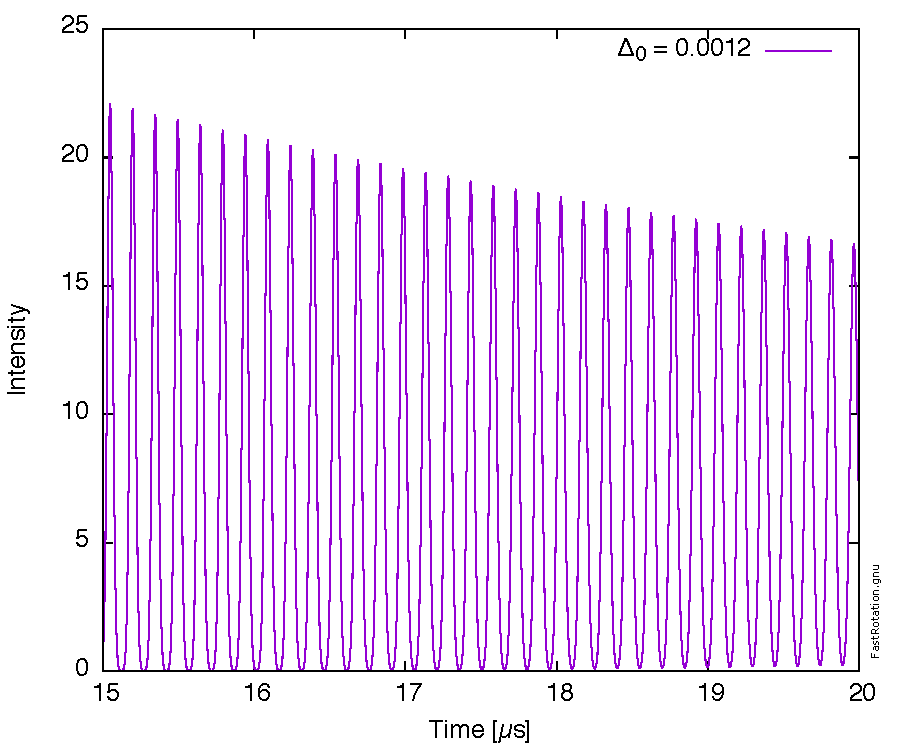
\includegraphics[trim = 0mm 0mm 0mm 0mm, clip=.false.,width=3.in]{/Users/dlr10/lepp/g-2/beamdynamics/damping_cbo/FastRotation_15-20.pdf} 
\caption{Fast rotation signal from 15$\mu$s to 20$\mu$s.
   \label{fig:fastrotation_15-20}}
\end{minipage}
\end{figure}
\subsection*{Momentum distribution from fast rotation signal}
The established method for extracting the energy (or equivalently frequency) distribution is to take the real part of the fourier transform of the fast rotation signal\cite{orlov},
\begin{eqnarray}
F(\omega,t_0) &=&\int_0^\infty S(t)\cos\omega(t-t_0) dt\nonumber\\
&=& \sum_{n=0}^\infty \int_0^\infty
\frac{e^{-(\frac{t}{nT}-1)^2/(2\Delta_0^2)}}{\sqrt{2\pi}\Delta_0 nT}\cos\omega(t-t_0) dt\nonumber\\
&=& \sum_{n=0}^\infty \int_0^\infty
\frac{e^{-t^2/(2(nT)^2\Delta_0^2)+t/(nT\Delta_0^2)\pm i\omega t}e^{\mp i\omega t_0}e^{-1/(2\Delta_0^2)}}{\sqrt{2\pi}\Delta_0 nT}\nonumber\\
&=& \frac{1}{2}\sum_{n=0}^\infty 
e^{(1/(nT\Delta_0^2)\pm i\omega t)^2)((nT)^2\Delta_0^2)/2}e^{\mp i\omega t_0}e^{-1/(2\Delta_0^2)}\nonumber\\
&=&\sum_{n=0}^\infty 
e^{(1/(nT\Delta_0^2)^2-(\omega t)^2))((nT)^2\Delta_0^2)/2}e^{-1/(2\Delta_0^2)}\cos\omega(nT-t_0)\nonumber\\
&=&\sum_{n=0}^\infty 
e^{(1/(2\Delta_0^2)-\omega ^2(nT)^2\Delta_0^2/2)}e^{-1/(2\Delta_0^2)}\cos\omega(nT-t_0)\nonumber\\
&=&\sum_{n=0}^\infty e^{-\omega^2(nT)^2\Delta_0^2/2}\cos\omega(nT-t_0)\label{eq:ftoffr}
\end{eqnarray}
\begin{figure}[htbp] %  figure placement: here, top, bottom, or page
\begin{minipage}[t]{0.48\textwidth}
   \centering
   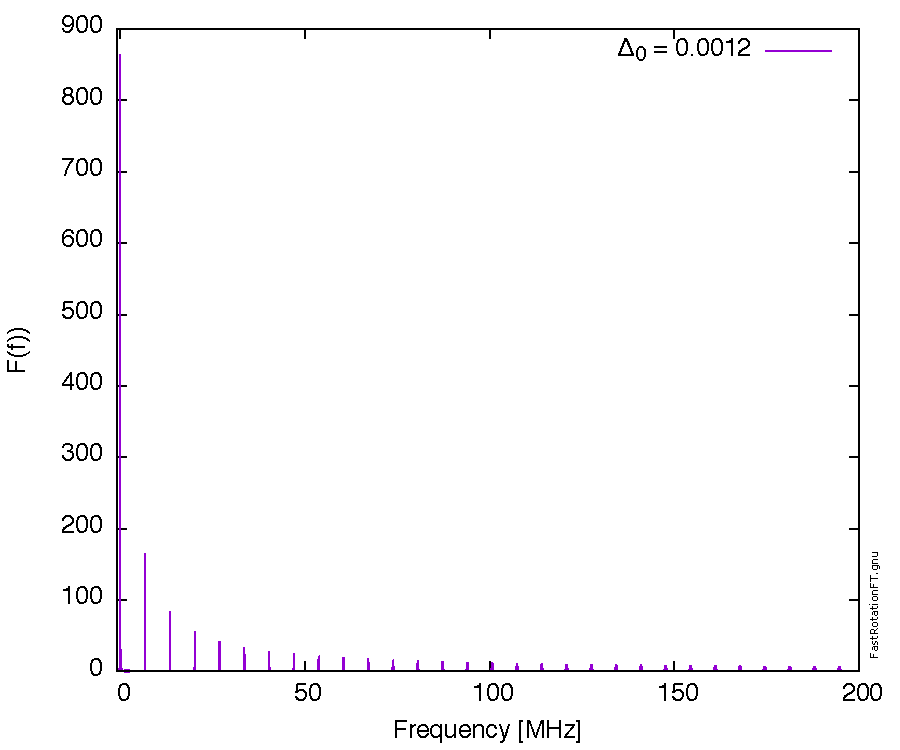
\includegraphics[trim = 0mm 0mm 0mm 0mm, clip=.false.,width=3.in]{/Users/dlr10/lepp/g-2/beamdynamics/damping_cbo/FastRotationFT_0-200.pdf} 
   \caption{Real part of fourier transform of fast rotation signal shown in Figure~\ref{fig:fastrotation_0-20}. \label{fig:fastrotationft_0-200}}
 \end{minipage}
\hfill
\begin{minipage}[t]{0.48\textwidth}
\centering
   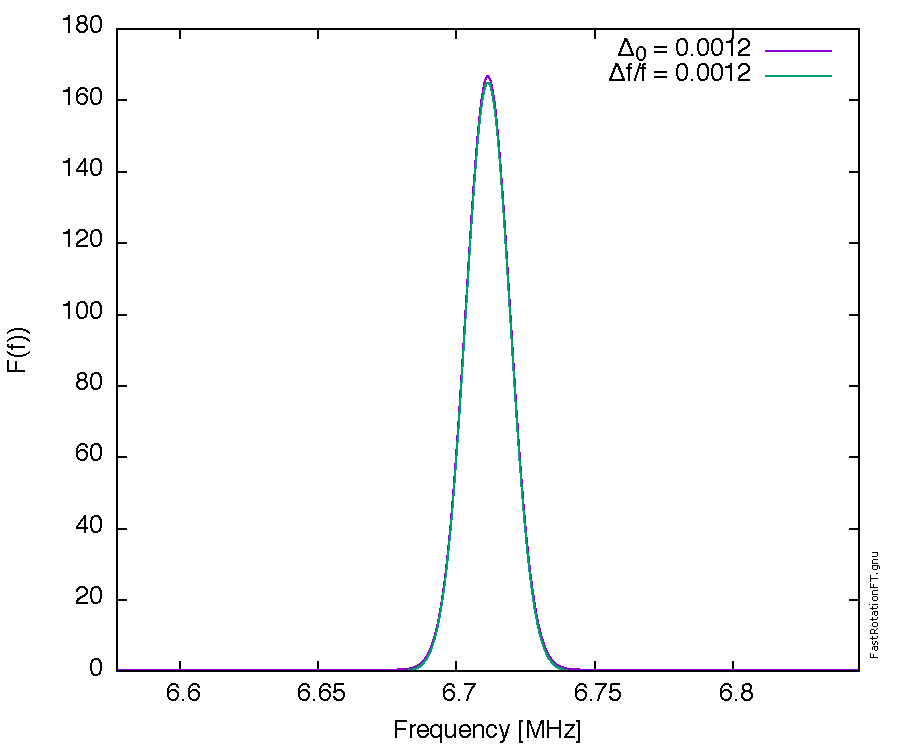
\includegraphics[trim = 0mm 0mm 0mm 0mm, clip=.false.,width=3.in]{/Users/dlr10/lepp/g-2/beamdynamics/damping_cbo/FastRotationFT_fit.pdf} 
\caption{Real part of fourier transform of fast rotation signal in Figure~\ref{fig:fastrotation_0-20} within the acceptance of the vacuum chamber. A Gaussian with
$\sigma_f/f = 0.0012$ is superimposed.
   \label{fig:fastrotationft_fit}}
\end{minipage}
\end{figure}

\section*{Bunch Length}
Next introduce finite bunch length. Referring back to Equation~\ref{eq:fr} it is straightforward to include a temporal offset $t^\prime$ as follows
\begin{eqnarray*}
S(t,t^\prime)&=& \sum_{n=0}^\infty\frac{e^{-(\frac{t-t^\prime}{nT}-1)^2/(2\Delta_0^2)}}{\sqrt{2\pi}\Delta_0 nT}
\end{eqnarray*}
Suppose the intial temporal (longitudinal) distribution of the muons is Gaussian $$\xi(t^\prime) = \frac{1}{\sqrt{2\pi}\sigma_t}e^{-{t^\prime}^2/(2\sigma_t^2)}$$
Then
\begin{eqnarray*}
S(t)&=& \sum_{n=0}^\infty\int_{-\infty}^\infty dt^\prime \frac{e^{-(\frac{t-t^\prime}{nT}-1)^2/(2\Delta_0^2)}}{\sqrt{2\pi}\Delta_0 nT}\frac{1}{\sqrt{2\pi}\sigma_t}e^{-{t^\prime}^2/(2\sigma_t^2)}
\\
&=& \sum_{n=0}^\infty\frac{1}{2\pi\Delta_0nT\sigma_t}\int_{-\infty}^\infty dt^\prime e^{-(\frac{t-t^\prime}{nT}-1)^2/(2\Delta_0^2)}e^{-{t^\prime}^2/(2\sigma_t^2)}\\
%&=& \sum_{n=0}^\infty\frac{1}{2\pi\Delta_0nT\sigma_t}e^{-t^2/(2(nT\Delta_0)^2)}
%\int_{-\infty}^\infty dt^\prime e^{-(\frac{{t^\prime}^2-2t t^\prime}{(nT)^2}+1 -\frac{2(t-t^\prime)}{nT})/(2\Delta_0^2)}e^{-{t^\prime}^2/(2\sigma_t^2)}\\
&=& \sum_{n=0}^\infty\frac{1}{2\pi\Delta_0nT\sigma_t}e^{-t^2/(2(nT\Delta_0)^2)}
\int_{-\infty}^\infty dt^\prime e^{-(\frac{{t^\prime}^2-2t t^\prime}{(nT)^2}+1 -\frac{2(t-t^\prime)}{nT})/(2\Delta_0^2)}e^{-{t^\prime}^2/(2\sigma_t^2)}\\
&=&\sum_{n=0}^\infty\frac{1}{2\pi\Delta_0nT\sigma_t}e^{-t^2/(2(nT\Delta_0)^2)}e^{\frac{t}{nT\Delta_0^2}}
\int_{-\infty}^\infty dt^\prime \exp(-{t^\prime}^2(\frac{1}{2(nT)^2\Delta_0^2}+\frac{1}{2\sigma_t^2})+t^\prime(\frac{t}{nT}-1)/(nT\Delta_0^2))e^{-1/(2\Delta_0^2)}\\
&=&\sum_{n=0}^\infty\frac{1}{2\pi\Delta_0nT\sigma_t}e^{-(\frac{t}{nT}-1)^2/2\Delta_0^2}
\int_{-\infty}^\infty dt^\prime \exp\left(-\alpha {t^\prime}^2+\beta t^\prime\right)\\
&=&\sum_{n=0}^\infty\frac{1}{2\pi\Delta_0nT\sigma_t}e^{-(\frac{t}{nT}-1)^2/(2\Delta_0^2)}
\sqrt{\frac{\pi}{\alpha}}e^{\beta^2/4\alpha}
\end{eqnarray*}
where $\alpha = \frac{1}{2(nT)^2\Delta_0^2}+\frac{1}{2\sigma_t^2}$ and $\beta= (\frac{t}{nT}-1)/(nT\Delta_0^2)$. 
Finally
\begin{eqnarray}
S(t)&=&\sum_{n=0}^\infty\frac{1}{2\pi\Delta_0nT\sigma_t}e^{-(\frac{t}{nT}-1)^2/(2\Delta_0^2)}
\frac{\sqrt{2\pi}nT\Delta_0\sigma_t}{\sqrt{(nT)^2\Delta_0^2+\sigma_t^2}}
\exp(\frac{(\frac{t}{nT}-1)^2}{(nT\Delta_0^2)^2}\frac{(nT)^2\Delta_0^2\sigma_t^2}{2(nT)^2\Delta_0^2+2\sigma_t^2})\nonumber\\
&=& \frac{1}{\sqrt{2\pi}}\sum_{n=0}^\infty e^{-(\frac{t}{nT}-1)^2/(2\Delta_0^2)}
\frac{1}{\sqrt{((nT)^2\Delta_0^2+\sigma_t^2}}
\exp(\frac{(\frac{t}{nT}-1)^2}{\Delta_0^2}\frac{\sigma_t^2}{2(nT)^2\Delta_0^2+2\sigma_t^2})\nonumber\\
&=& \frac{1}{\sqrt{2\pi}}\sum_{n=0}^\infty
\frac{1}{\sqrt{((nT)^2\Delta_0^2+\sigma_t^2}}
\exp(\frac{-(\frac{t}{nT}-1)^2}{2\Delta_0^2}\left(1-\frac{\sigma_t^2}{(nT)^2\Delta_0^2+\sigma_t^2}\right))\label{eq:frs-sigt}
\end{eqnarray}
Check the limits
\begin{eqnarray*}
S(t)\lim_{\sigma_t\rightarrow 0} &=& \sum_{n=0}^\infty e^{(\frac{t}{nT}-1)^2/(2\Delta_0^2)}
\frac{1}{\sqrt{2\pi}(nT)\Delta_0}
\end{eqnarray*}
In the limit where $\sigma_t \gg nT\Delta_0$
\begin{eqnarray*}
S(t)\lim_{\sigma_t\rightarrow \infty} &=& 
 \sum_{n=0}^\infty e^{-(\frac{t}{nT}-1)^2/(2\Delta_0^2)}
\frac{1}{\sqrt{2\pi((nT)^2\Delta_0^2+\sigma_t^2}}
\exp(\frac{(\frac{t}{nT}-1)^2}{2\Delta_0^2})\\
&\sim& \sum_{n=0}^{\frac{\sigma_t}{T\Delta_0}}
\frac{1}{\sqrt{2\pi}\sigma_t}\\
&=& \frac{\sigma_t}{T\Delta_0}(\frac{\sigma_t}{T\Delta_0} + 1)\frac{1}{\sqrt{2\pi}\sigma_t}\\
&\sim& \frac{\sigma_t}{\sqrt{2\pi}T^2\Delta_0^2}
\end{eqnarray*}
and the signal is independent of time.
Let's look at a couple of examples.
Figure~\ref{fig:fastrotation_sigt20ns} shows the first 20 $\mu$s of the fast rotation signal
of a distribution with Gaussian energy spread $\Delta E/E=0.0012$ and pulse length $\sigma_t=$20ns. This is to 
be compared with Fig.~\ref{fig:fastrotation_0-20} with $\sigma_t=0$. Figure~\ref{fig:fastrotation_sigt60ns} is the fast rotation
signal for a distribution with the same energy spread but pulse length $\sigma_t=60$ns, closer to what we will see in E989. 
\begin{figure}[htbp] %  figure placement: here, top, bottom, or page
\begin{minipage}[t]{0.48\textwidth}
   \centering
   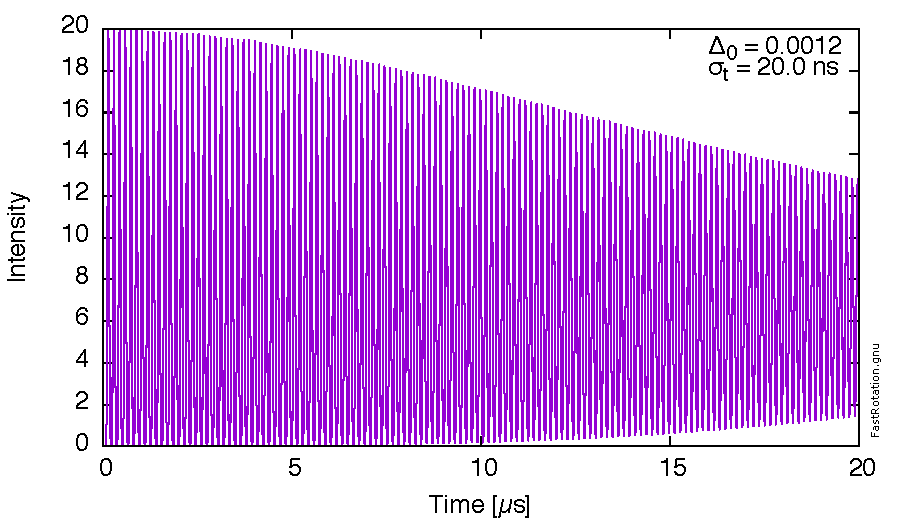
\includegraphics[trim = 0mm 0mm 0mm 0mm, clip=.false.,width=3.in]{/Users/dlr10/lepp/g-2/beamdynamics/damping_cbo/FastRotation_0-20_st20.pdf} 
   \caption{Fast rotation signal from a muon pulse with Gaussian energy spread $\Delta E/E=0.0012$ and 
Gaussian temporal spread $\sigma_t = 20$ns. \label{fig:fastrotation_sigt20ns}}
 \end{minipage}
\hfill
\begin{minipage}[t]{0.48\textwidth}
\centering
   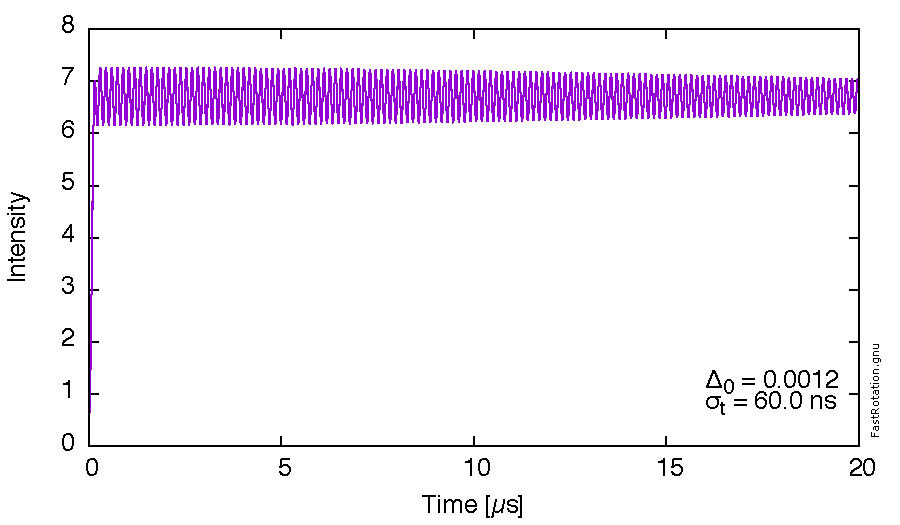
\includegraphics[trim = 0mm 0mm 0mm 0mm, clip=.false.,width=3.in]{/Users/dlr10/lepp/g-2/beamdynamics/damping_cbo/FastRotation_0-20_st60.pdf} 
\caption{Fast rotation signal from muon pulse with $\Delta E/E = 0.0012$, and $\sigma_t = 60$ns.
   \label{fig:fastrotation_sigt60ns}}
\end{minipage}
\end{figure}
It will turn out to be convenient to rewrite Equation~\ref{eq:frs-sigt} as
\begin{eqnarray}
S(t)&=& \frac{1}{\sqrt{2\pi}}\sum_{n=0}^\infty
\frac{1}{\sqrt{((nT)^2{\Delta^\prime_0}^2}}
\exp(\frac{-(\frac{t}{nT}-1)^2}{2{\Delta^\prime_0}^2})\label{eq:frs-sigt-dp}
\end{eqnarray}
where $${\Delta^\prime_0}^2 = \frac{(nT\Delta_0)^2+\sigma_t^2}{(nT)^2}$$
Then it is easy to see that the Fourier transform has the same form as Equation~\ref{eq:ftoffr} and
\begin{eqnarray*}
F(\omega,t_0,\Delta_0^\prime)&=& \sum_{n=0}^\infty e^{-\omega^2(nT)^2{\Delta_0^\prime}^2/2}\cos\omega(nT-t_0)
\end{eqnarray*}
Examples of fourier transforms (Equation~\ref{eq:frs-sigt-dp}) of the fast rotation signal for distributions with energy width $\Delta E/E=0.0012$ and
lengths $\sigma_t=20$ns and $\sigma_t=60$ ns respectively are shown in Figure~\ref{fig:ft-sigt20-60}
over the frequency range consistent with the chamber aperture. For both cases the the distribution is Gaussian with width $\Delta f/f = 0.0012$ so that the Fourier
transform does indeed reproduce the energy spread. The effect of the bunch length is to reduce the amplitude of the signal. At what point the signal is dominated by statistical noise remains to be determined. 
\begin{figure}[htbp]
\centering
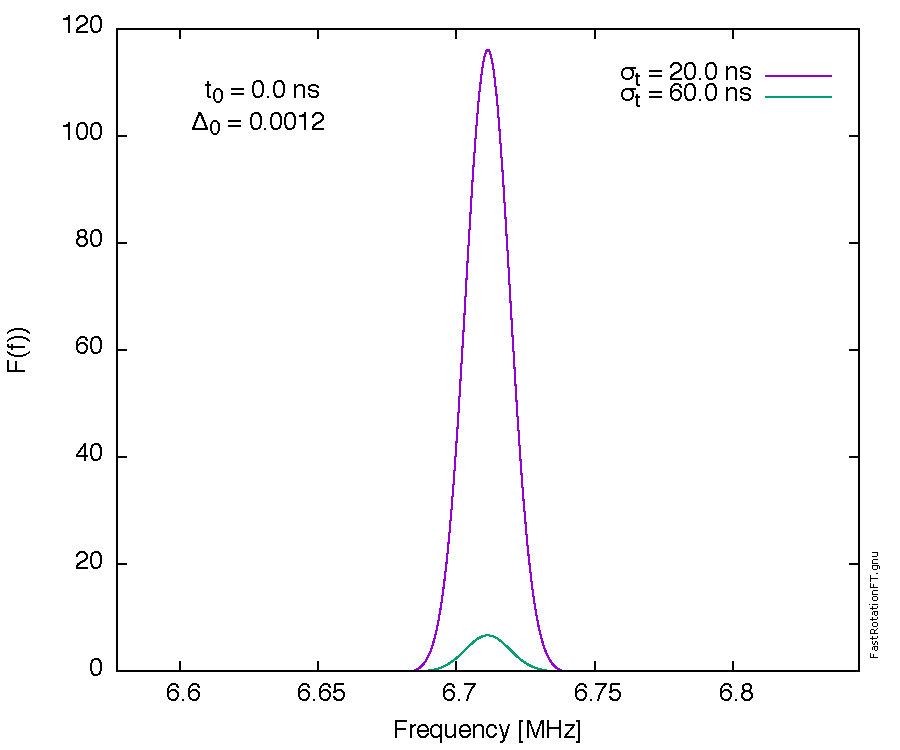
\includegraphics[width=4in]{/Users/dlr10/lepp/g-2/beamdynamics/damping_cbo/FastRotationFT_sigt20-sigt60ns.pdf}
\caption{Fourier transform of fast rotation signal for distributions with pulse length $\sigma_t=20$ns and $\sigma_t=60$ns.
\label{fig:ft-sigt20-60}}
\end{figure}
\section*{Energy and dispersion}
The final focus of the M5 line is designed so that the dispersion at the
exit of the inflector is zero\cite{rubin} so the muons entering the ring with fractional energy offset $\Delta$, 
will oscillate transversely about their closed orbit $(x_c(\Delta)=\eta\Delta)$ with 
amplitude $x(\Delta)=\eta\Delta$ and frequency 
%If we turn off quad nonlinearities
$$ f=Q\omega_0 \rightarrow (Q+Q^\prime\Delta)\frac{\omega_0}{1+\Delta}$$
where $\omega_0$ is the revolution frequency of the magic momentum muon, and $Q$ and $Q^\prime$ are the
horizontal betatron tune and chromaticity respectively.
The transverse motion of a single muon with energy offset $\Delta$ is
$$x(t) = \eta\Delta(1-\cos\left((Q+Q^\prime\Delta)\frac{\omega_0 t}{1+\Delta} \right)$$
Then the position at the fixed point $s$ is
$$x(t,\Delta)_s = \sum_n\eta\Delta\left(1-\cos\left( (Q+Q^\prime\Delta)\frac{\omega_0}{1+\Delta}   t\right)\right)\delta(t-nT(1+\Delta))$$
$$x(t,\Delta)_s = \sum_n\eta\Delta\left(1-\cos\left((Q+Q^\prime\Delta)\frac{\omega_0}{1+\Delta} t\right)\right)\delta(\Delta - (\frac{t}{nT}-1))$$
Next consider a distribution with zero emittance and zero length, but finite Gaussian energy spread,
$$\rho(\Delta) = \frac{e^{-\frac{\Delta^2}{\Delta_0^2}}}{\sqrt{2\pi}\Delta_0}$$ 
Averaging over all energy offsets we find
\begin{eqnarray*}
N\langle x(t)\rangle &=&
\int_{-\infty}^\infty d\Delta\sum_n\eta\Delta(\left(1-\cos\left((Q+Q^\prime\Delta)\frac{\omega_0}{1+\Delta} t\right)\right)\frac{e^{-\frac{\Delta^2}{2\Delta_0^2}}}{\sqrt{2\pi}\Delta_0}\delta(\Delta-(\frac{t}{nT}-1))\\
&=&
\sum_n\eta(\frac{t}{nT}-1)\left(1-\cos\left((Q+ Q^\prime(\frac{t}{nT}-1))\frac{\omega_0}{t/nT} t\right)\right)\frac{e^{-\frac{(\frac{t}{nT}-1)^2}{2\Delta_0^2}}}{\sqrt{2\pi}\Delta_0}\\
&=&\sum_n\eta(\frac{t}{nT}-1)\left(1-\cos\left((QnT+ Q^\prime(t-nT))\omega_0 \right)\right)\frac{1}{\sqrt{2\pi}\Delta_0}e^{-\frac{(\frac{t}{nT}-1)^2}{2\Delta_0^2}}
\end{eqnarray*}
$N\langle x(t)\rangle$ is the average position at time $t$, weighted by the number of muons at that time.
In order to extract the average position, divide by
$$N = \sum_n \frac{1}{\sqrt{2\pi}\Delta_0}e^{-\frac{(\frac{t}{nT}-1)}{2\Delta_0^2}}$$
so that
\begin{equation}
\langle x(t)\rangle = \frac{1}{N}
\sum_n\eta(\frac{t}{nT}-1)\left(1-\cos\left((QnT+ Q^\prime(t-nT))\omega_0 \right)\right)\frac{1}{\sqrt{2\pi}\Delta_0}e^{-\frac{(\frac{t}{nT}-1)^2}{2\Delta_0^2}}\label{eq:averagex}
\end{equation}
The average centroid displacement at a fixed point in the ring (for example at a fiber harp) is given by Equation~\ref{eq:averagex} and plotted in Figure~\ref{fig:EnergyDecoherence_160ms} for an initial distribution with Gaussian energy width $\Delta_0=0.0012$, zero pulse length and zero emittance. The betatron motion decoheres on a time scale of 30$\mu$s.
The frequency of the envelope of the turn by turn motion, most apparent in the first 20$\mu$s (Fig.~\ref{fig:EnergyDecoherence_20}) is the betatron tune $(f_\beta = Q\omega_0$).   
A coherent oscillation of the centroid persists beyond 100$\mu$s (Fig.~\ref{fig:EnergyDecoherence_40-100}.)
\begin{figure}[htbp]
%\begin{minipage}[t]{0.48\textwidth}
\centering
   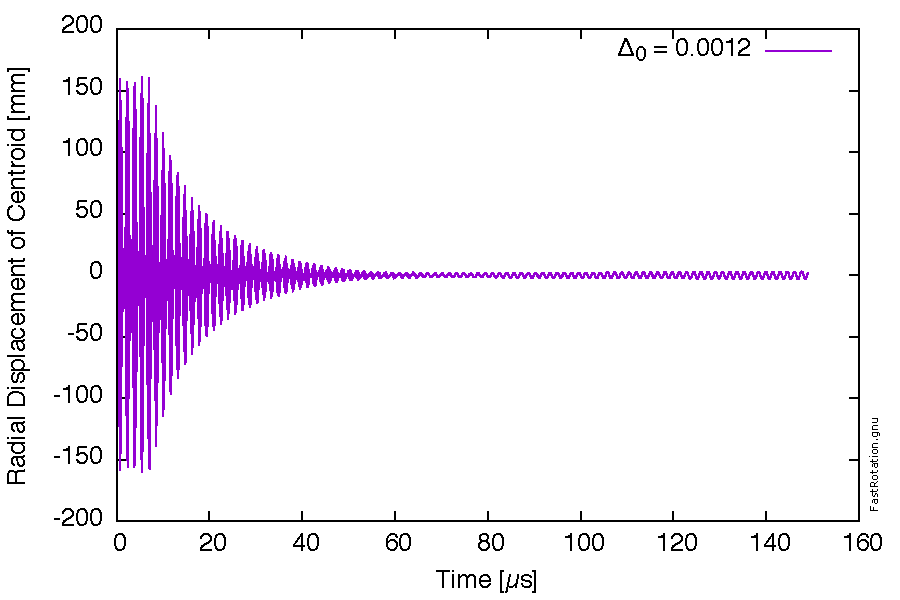
\includegraphics[trim = 0mm 0mm 0mm 0mm, clip=.false.,width=4.5in]{/Users/dlr10/lepp/g-2/beamdynamics/damping_cbo/EnergyDecoherence_0-160.pdf} 
\caption{Centroid motion of a distribution with Gaussian energy distribution, zero length and emittance
   \label{fig:EnergyDecoherence_160ms}}
%\end{minipage}
\end{figure}
\begin{figure}[htbp] %  figure placement: here, top, bottom, or page
\begin{minipage}[t]{0.48\textwidth}
   \centering
   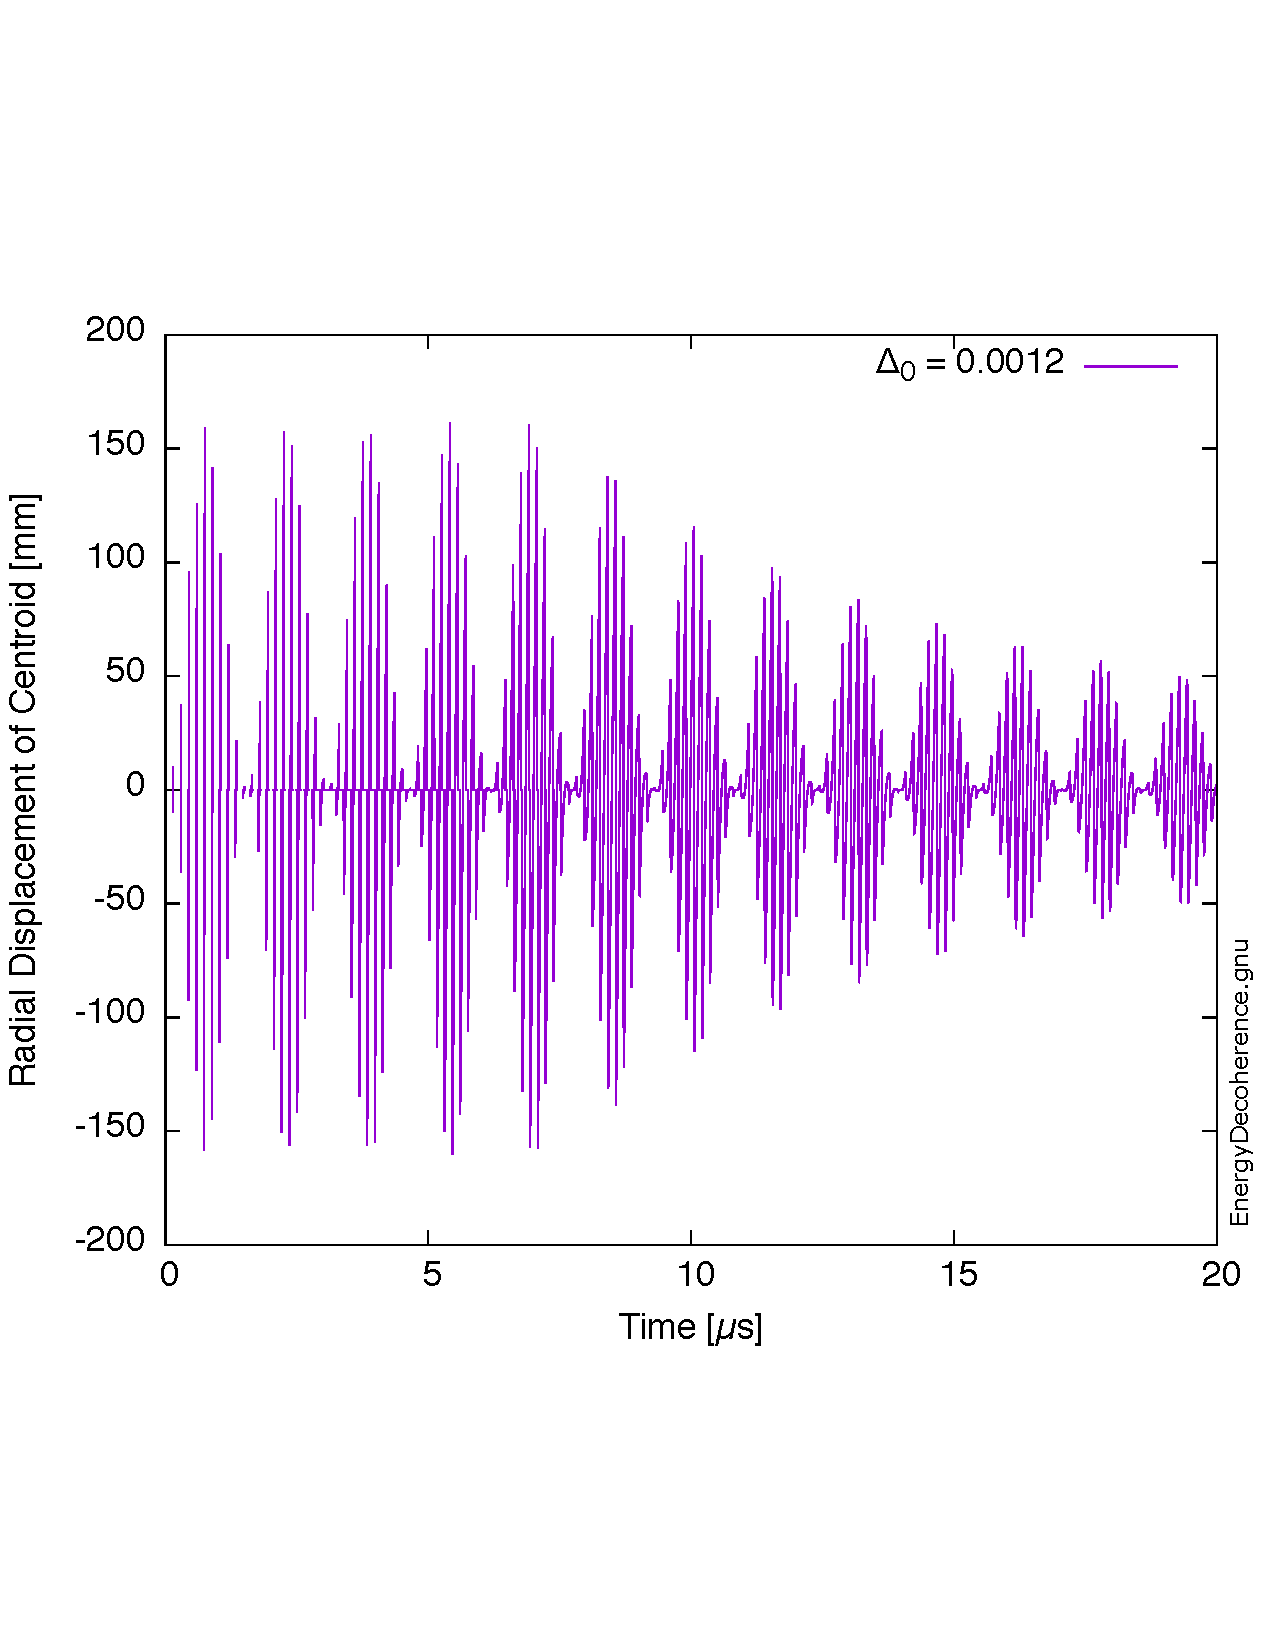
\includegraphics[trim = 0mm 0mm 0mm 0mm, clip=.false.,width=3.in]{/Users/dlr10/lepp/g-2/beamdynamics/damping_cbo/EnergyDecoherence_20ms.pdf} 
   \caption{Centroid motion for the same distribution as Fig. \ref{fig:EnergyDecoherence_160ms} for the first 20$\mu$s after injection. The
frequency of the envelope is the betatron tune. \label{fig:EnergyDecoherence_20}}
 \end{minipage}
\hfill
\begin{minipage}[t]{0.48\textwidth}
\centering
   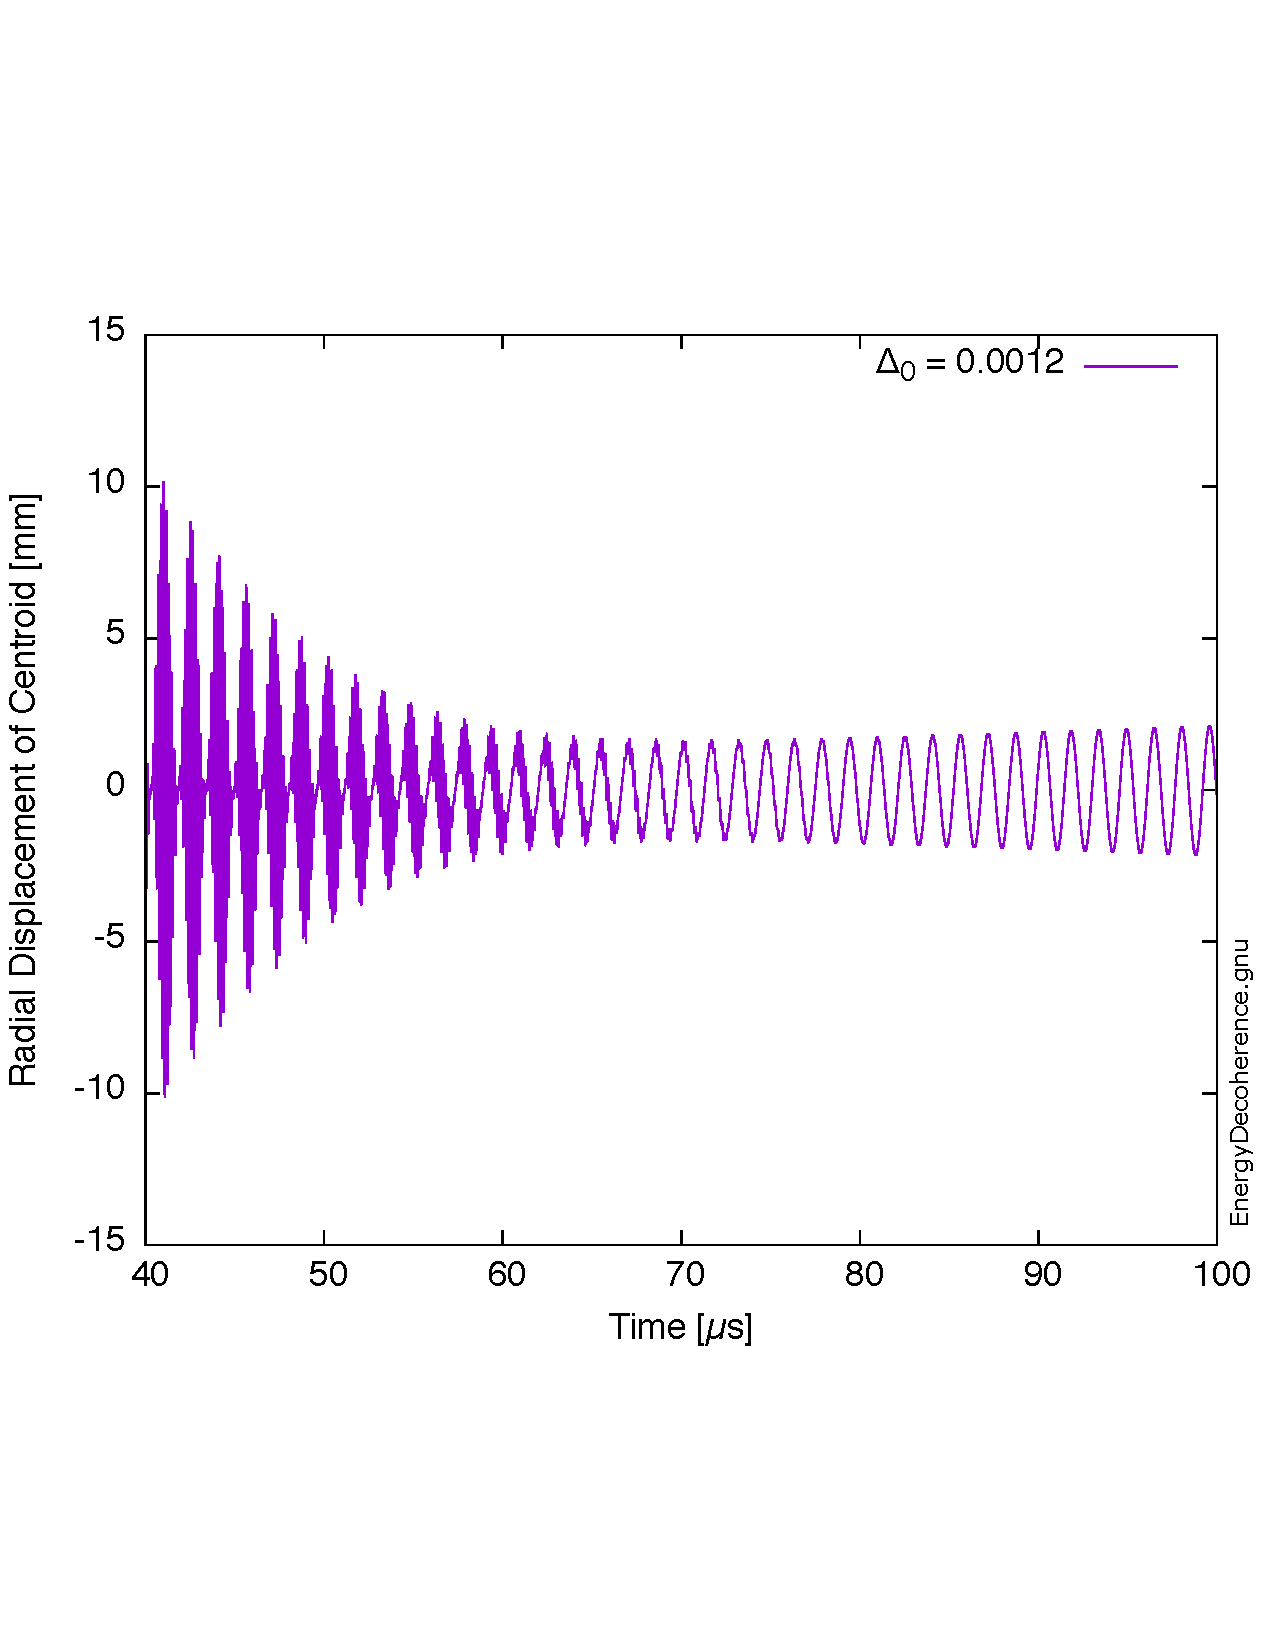
\includegraphics[trim = 0mm 0mm 0mm 0mm, clip=.false.,width=3.in]{/Users/dlr10/lepp/g-2/beamdynamics/damping_cbo/EnergyDecoherence_40-100ms.pdf} 
\caption{Centroid motion for the same distribution as Fig.~\ref{fig:EnergyDecoherence_160ms} 40-100$\mu$s after injection.
   \label{fig:EnergyDecoherence_40-100}}
\end{minipage}
\end{figure}
%

We can reproduce the analytic result in a tracking simulation. Figures~\ref{fig:TimeDepMom_145}-~\ref{fig:TimeDepMom_130-145} are simulation data
with the BMAD model of the storage ring, including collimators and quadrupole nonlinearity (which are of course no part of the analytic calcuation). 
The distribution 
has Gaussian energy width $\Delta E/E=\Delta_0$, pulse length
$\sigma_t=1$ns (that is, approximately zero) and zero emittance. The muon distribution is injected on axis, mimicing a perfect kick. Nevertheless, 
a coherent betatron oscillation emerges as the envelope of the fast rotation signal. Immediatelay after injection, there is zero coherent oscillation.
As long as the average momentum is the magic momentum, the average displacement is zero. The betatron oscillations of the high and low momentum muons
are 180 deg out of phase. Coherent oscillations appear as the high momentum muons lag behind the low momentum particles. Also, because
the momentum spread of the distribution at the inflector exit is greater than the momentum acceptance of the ring, the amplitude of the coherent oscillations
arising from the momentum spread will by definition fill the aperture. One thing to keep in mind: the time dependence of the centroid motion at a fixed point
in the ring as shown in Figures~\ref{fig:TimeDepMom_145}-~\ref{fig:TimeDepMom_130-145}, etc. will depend on the width of the time bin, which here is 1ns. 
As the width of the time bin increases the average displacement of the distribution decreases, approaching zero as the time bin approaches the revolution period of 
149 ns. Note also that each point in the Figures will in general correpond to the average of the positions of only those muons
in that particular time bin. As a result, some points will represent the average of a very few muons. It
is a plot of average position versus time, with no accounting for intensity.
%
\begin{figure}[htbp] %  figure placement: here, top, bottom, or page
\begin{minipage}[t]{0.48\textwidth}
   \centering
   \includegraphics[trim = 0mm 0mm 0mm 0mm, clip=.false.,width=3.in]{/Users/dlr10/development/bmad_dist/g-2/damping/20160711_123314/Time_Dep_Moments_x_0-145.pdf} 
   \caption{Centroid motion for a distribution with Gaussian energy width $\Delta E/E=0.0012$, zero length, and zero emittance. The distribution
is injected on axis into the ring, so that there is initially no coherent betatron oscillation. Centroid motion evolves
with time due to the momentum spread.\label{fig:TimeDepMom_145}}
 \end{minipage}
\hfill
\begin{minipage}[t]{0.48\textwidth}
\centering
   \includegraphics[trim = 0mm 0mm 0mm 0mm, clip=.false.,width=3.in]{/Users/dlr10/development/bmad_dist/g-2/damping/20160711_123314/Time_Dep_Moments_x_0-20.pdf} 
\caption{Centroid motion for the same distribution as Fig.~\ref{fig:TimeDepMom_145} for the first 20$\mu$s after injection. The coherent oscillation of the centroid
is evident. The centroid motion is modulated at the betatron tune.
\label{fig:TimeDepMom_0-20}}
\end{minipage}
\end{figure}
It is clear again in Fig.~\ref{fig:TimeDepMom_130-145} that a coherent oscillation persists well beyond 100 $\mu$s, albeit with relatively small amplitude
of $\pm 5$mm.
\begin{figure}[htbp] %  figure placement: here, top, bottom, or page
\begin{minipage}[t]{0.48\textwidth}
   \centering
   \includegraphics[trim = 0mm 0mm 0mm 0mm, clip=.false.,width=3.in]{/Users/dlr10/development/bmad_dist/g-2/damping/20160711_123314/Time_Dep_Moments_x_30-60.pdf} 
   \caption{Centroid motion for the same distribution as Fig.~\ref{fig:TimeDepMom_145} from 30-60$\mu$s after injection. The
decoherence time is about $30\mu$s. \label{fig:TimeDepMom_30-60}}
 \end{minipage}
\hfill
\begin{minipage}[t]{0.48\textwidth}
\centering
   \includegraphics[trim = 0mm 0mm 0mm 0mm, clip=.false.,width=3.in]{/Users/dlr10/development/bmad_dist/g-2/damping/20160711_123314/Time_Dep_Moments_x_130-145.pdf} 
\caption{Centroid motion for the same distribution as Fig.~\ref{fig:TimeDepMom_145} 130-145$\mu$s after injection. Some coherent motion persists well beyond $100\mu$s.
   \label{fig:TimeDepMom_130-145}}
\end{minipage}
\end{figure}

\section{Put the pieces together}
What happens if there is finite energy spread, 40mm-mrad emittance, and finite pulse length, namely anticipated 989 W?%20160710_193840



\begin{figure}[htbp] %  figure placement: here, top, bottom, or page
\begin{minipage}[t]{0.48\textwidth}
   \centering
   \includegraphics[trim = 0mm 0mm 0mm 0mm, clip=.false.,width=3.in]{/Users/dlr10/development/bmad_dist/g-2/damping/20160711_153147/Time_Dep_Moments_x_0-145.pdf} 
   \caption{Finite emittance and W pulse shape, energy spread = 0.0012\label{fig:20160711_153147-finite-emit-tau-energy_0-145}}
 \end{minipage}
\hfill
\begin{minipage}[t]{0.48\textwidth}
   \centering
   \includegraphics[trim = 0mm 0mm 0mm 0mm, clip=.false.,width=3.in]{/Users/dlr10/development/bmad_dist/g-2/damping/20160711_153147/Time_Dep_Moments_x_0-20.pdf} 
   \caption{Finite emittance and W pulse shape, energy spread\label{fig:20160711_153147-finite-emit-tau-energy_0-20}}
 \end{minipage}
\end{figure}
\begin{figure}[htbp] %  figure placement: here, top, bottom, or page
\begin{minipage}[t]{0.48\textwidth}
   \centering
   \includegraphics[trim = 0mm 0mm 0mm 0mm, clip=.false.,width=3.in]{/Users/dlr10/development/bmad_dist/g-2/damping/20160711_153147/Time_Dep_Moments_x_30-60.pdf} 
   \caption{Finite emittance and W pulse shape, energy spread = 0.0012\label{fig:20160711_153147-finite-emit-tau-energy_0-145}}
 \end{minipage}
\hfill
\begin{minipage}[t]{0.48\textwidth}
   \centering
   \includegraphics[trim = 0mm 0mm 0mm 0mm, clip=.false.,width=3.in]{/Users/dlr10/development/bmad_dist/g-2/damping/20160711_153147/Time_Dep_Moments_x_130-145.pdf} 
   \caption{Finite emittance and W pulse shape, energy spread\label{fig:20160711_153147-finite-emit-tau-energy_130-145}}
 \end{minipage}
\end{figure}

Let's try one more thing. Suppose the kick is imperfect and there is some displacement or angle of the injected muons with respect to the closed orbit
and a coherent oscillation of the centroid.
\begin{figure}[htbp] %  figure placement: here, top, bottom, or page
\begin{minipage}[t]{0.48\textwidth}
   \centering
   \includegraphics[trim = 0mm 0mm 0mm 0mm, clip=.false.,width=3.in]{/Users/dlr10/development/bmad_dist/g-2/damping/20160711_205325/Time_Dep_Moments_x_20-60.pdf} 
   \caption{Finite emittance and W pulse shape, energy spread = 0.0012\label{fig:20160711_205325-finite-emit-tau-energy_0-20}}
 \end{minipage}
\hfill
\begin{minipage}[t]{0.48\textwidth}
   \centering
   \includegraphics[trim = 0mm 0mm 0mm 0mm, clip=.false.,width=3.in]{/Users/dlr10/development/bmad_dist/g-2/damping/20160711_205325/Time_Dep_Moments_x_130-145.pdf} 
   \caption{Finite emittance and W pulse shape, energy spread\label{fig:20160711_205325-finite-emit-tau-energy_130-145}}
 \end{minipage}
\end{figure}

%\begin{eqnarray*}
%\langle x \rangle &=& x(\Delta)\left(\cos(Q\omega_0 t)\langle\cos(Q^\prime-Q)\Delta\omega_0 t\rangle
%-\sin Q\omega_0 t \langle \sin(Q^\prime-Q)\delta\omega_0 t\rangle\right)\\
% &=& \eta\left(\cos(Q\omega_0 t)\sum_{\delta_i}\delta_i\cos(Q^\prime-Q)\delta_i\omega_0 t
%-\sin Q\omega_0 t\sum_{\delta_i}\delta_i \sin(Q^\prime-Q)\delta\omega_0 t\right)\\
%\end{eqnarray*}
%The first term vanishes as $\delta_i$ is asymmetric about zero and cos is symmetric.
%Then
%\begin{eqnarray*}
%\langle x \rangle &=& -\eta\sin Q\omega_0 t \frac{1}{2i\sqrt{2\pi}\delta_0}\int_{-\infty}^\infty \delta \left(e^{i\xi\delta}-e^{-i\xi\delta}\right)e^{-\frac{1}{2}\frac{\delta^2}{\delta_0^2}}\\
% &=& -\eta\sin Q\omega_0 t \frac{1}{2i\sqrt{2\pi}\delta_0}\frac{1}{i}\der{}{\xi}\int_{-\infty}^\infty  \left(e^{i\xi\delta}+e^{-i\xi\delta}\right)e^{-\frac{1}{2}\frac{\delta^2}{\delta_0^2}}\\
% &=& -\eta\sin Q\omega_0 t \frac{2}{2i\sqrt{2\pi}\delta_0}\frac{1}{i}\der{}{\xi}e^{-\frac{1}{2}\xi^2\delta_0^2}(\sqrt{2\pi}\delta_0)\\
% &=& \eta\sin Q\omega_0 t \der{}{\xi}e^{-\frac{1}{2}\xi^2\delta_0^2}\\
% &=& -\eta\sin (Q\omega_0 t) \xi\delta_0^2e^{-\frac{1}{2}\xi^2\delta_0^2}\\
%\end{eqnarray*}

\newpage
\section*{Appendix}
The real part of the Fourier transform of the fast rotation signal of a Gaussian distribution of energies with $\sigma_E/E = 0.0012$ is given by
\begin{equation}
F(\omega, \Delta_0,t_0)=\sum_{n=0}^\infty e^{-\omega^2(nT)^2\Delta_0^2/2}\cos\omega(nT-t_0)\label{eq:ftfr}
\end{equation}
$F(\omega,\Delta_0,t_0)$ for a various values of the start time offset $t_0$ are shown in Figures~\ref{fig:fastrotationft_fit_t00} -~\ref{fig:fastrotationft_fit_t05}.
\begin{figure}[htbp] %  figure placement: here, top, bottom, or page
\begin{minipage}[t]{0.32\textwidth}
   \centering
   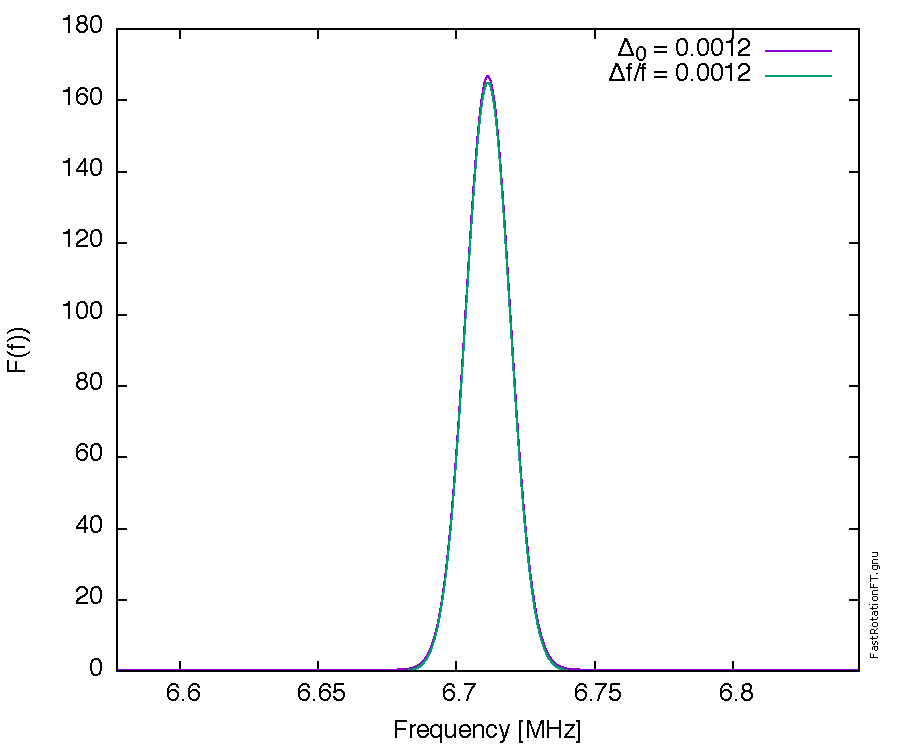
\includegraphics[trim = 0mm 0mm 0mm 0mm, clip=.false.,width=2.in]{/Users/dlr10/lepp/g-2/beamdynamics/damping_cbo/FastRotationFT_fit.pdf} 
   \caption{Real part of fourier transform of fast rotation signal shown in Figure~\ref{fig:fastrotation_0-20}. Gaussian with width $\Delta f/f=0.0012$ 
is superimposed. $t_0=0$. \label{fig:fastrotationft_fit_t00}}
 \end{minipage}
\hfill
\begin{minipage}[t]{0.32\textwidth}
\centering
   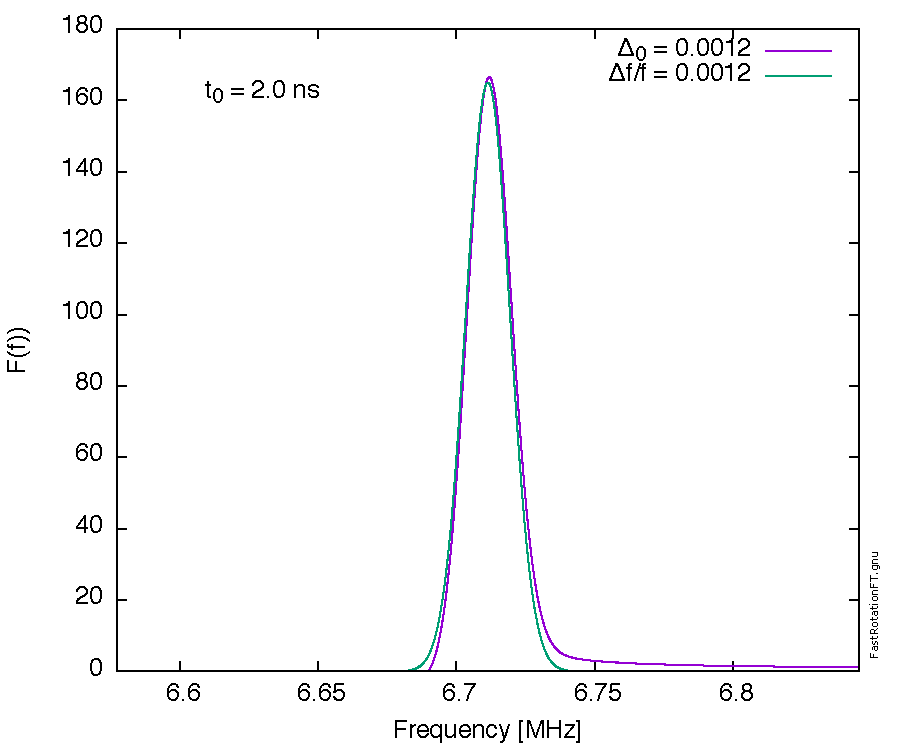
\includegraphics[trim = 0mm 0mm 0mm 0mm, clip=.false.,width=2.in]{/Users/dlr10/lepp/g-2/beamdynamics/damping_cbo/FastRotationFT_fit_t02.pdf} 
\caption{Same as Figure~\ref{fig:fastrotationft_fit_t02} but with $t_0=2$ns (see Equation~\ref{eq:ftfr}).
   \label{fig:fastrotationft_fit_t02}}
\end{minipage}
\hfill
\begin{minipage}[t]{0.32\textwidth}
\centering
   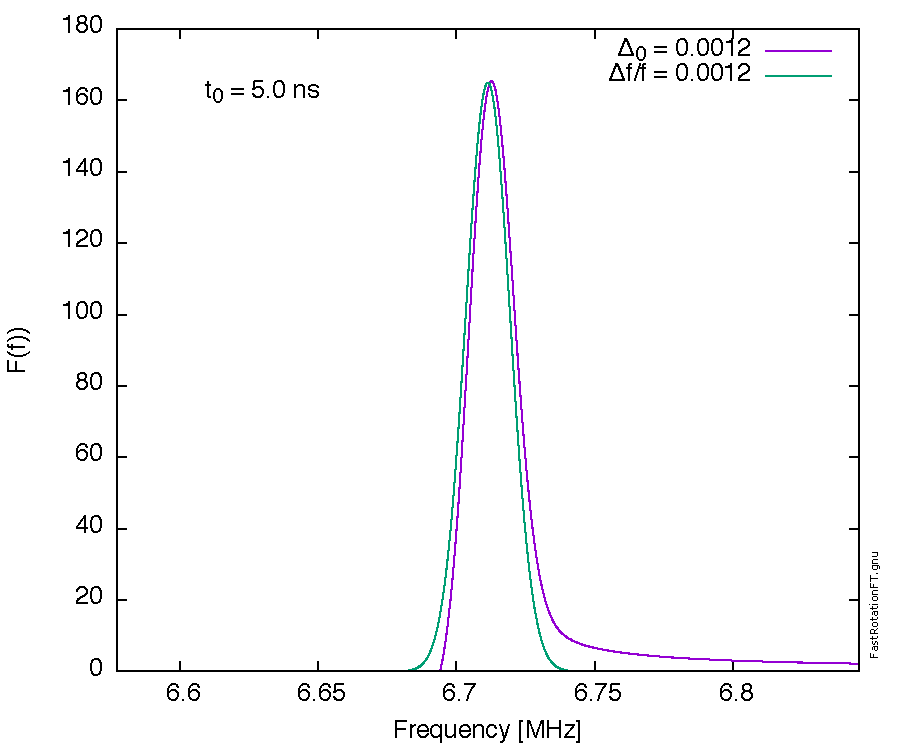
\includegraphics[trim = 0mm 0mm 0mm 0mm, clip=.false.,width=2.in]{/Users/dlr10/lepp/g-2/beamdynamics/damping_cbo/FastRotationFT_fit_t05.pdf} 
\caption{Same as Figure~\ref{fig:fastrotationft_fit_t05} but with $t_0=5$ns.
   \label{fig:fastrotationft_fit_t05}}
\end{minipage}
\end{figure}



\begin{thebibliography}{9}

\bibitem{NIMesquad}
Yannis K. Semertzidis, Gerald Bennett, Efstratios Efstathiadis, Frank Krienen, Richard Larsen, Y.Y. Lee, William M. Morse, 
Yuri Orlov, Cenap S. Ozben, B. Lee Roberts, Louis P. Snydstrup, David S. Warburton.
\textit{The Brookhaven muon (g-2) storage ring high voltage quadrupole}.
Nuclear Instruments and Methods in Physics Research A 503 (2003) 458–484


\bibitem{orlov}
Yuri Orlov, Cenap S. Ozben, and Yannis K. Semertzidis.
\textit{Muon revolution frequency distribution from a partial-time Fourier transform of the g-2 signal in the muon g-2 experiment}.
Nuclear Instruments and Methods in Physics Research A 482 (2002) 767–775

\bibitem{rubin}
D. Rubin. \textit{Beam Dynamics Injectionand Storage}. G-2 Experiment Document 2820-v5
\end{thebibliography}
\end{document}

-------------------------------------------------
with a change of index from 0.185 to 0.18, (no multipoles) the first node is at 350 turns

Analytic Delta Qx/Delta index = (0.90597-0.91677)/0.02 = -0.54
Therefore expect Delta Qx = 0.005*-0.54=0.0027 = 1/370.



\section{Energy dependent tune}
The betatron tune depends on the energy of the particle. The chromaticities
$$Q^\prime_h = -0.14,\ \ \ \ Q^\prime_v = 0.31$$ 
Then the energy dependent tune shift is
$$\Delta Q = Q^\prime \sigma_E$$

$$U =\sum_{n=0} r^n [a_n \sin(n\phi) +b_n  \cos(n\phi)]$$
$$E_x=-{\bf \nabla} U = \sum_n n r^{n-1}[a_n \sin(n\phi) + b_n  \cos(n\phi)]$$
and at $\phi=0$
$$E_x=-{\bf \nabla} U = -\sum_n n x^{n-1}b_n$$
$$\der{E_x}{x} = \sum_n n(n-1) x^{n-2}b_n$$
$$U=b_1 x + b_2 x^2 +b_3 x^3 +b_4 x^4$$



\begin{figure}[htbp] %  figure placement: here, top, bottom, or page
\begin{minipage}[t]{0.48\textwidth}
   \centering
   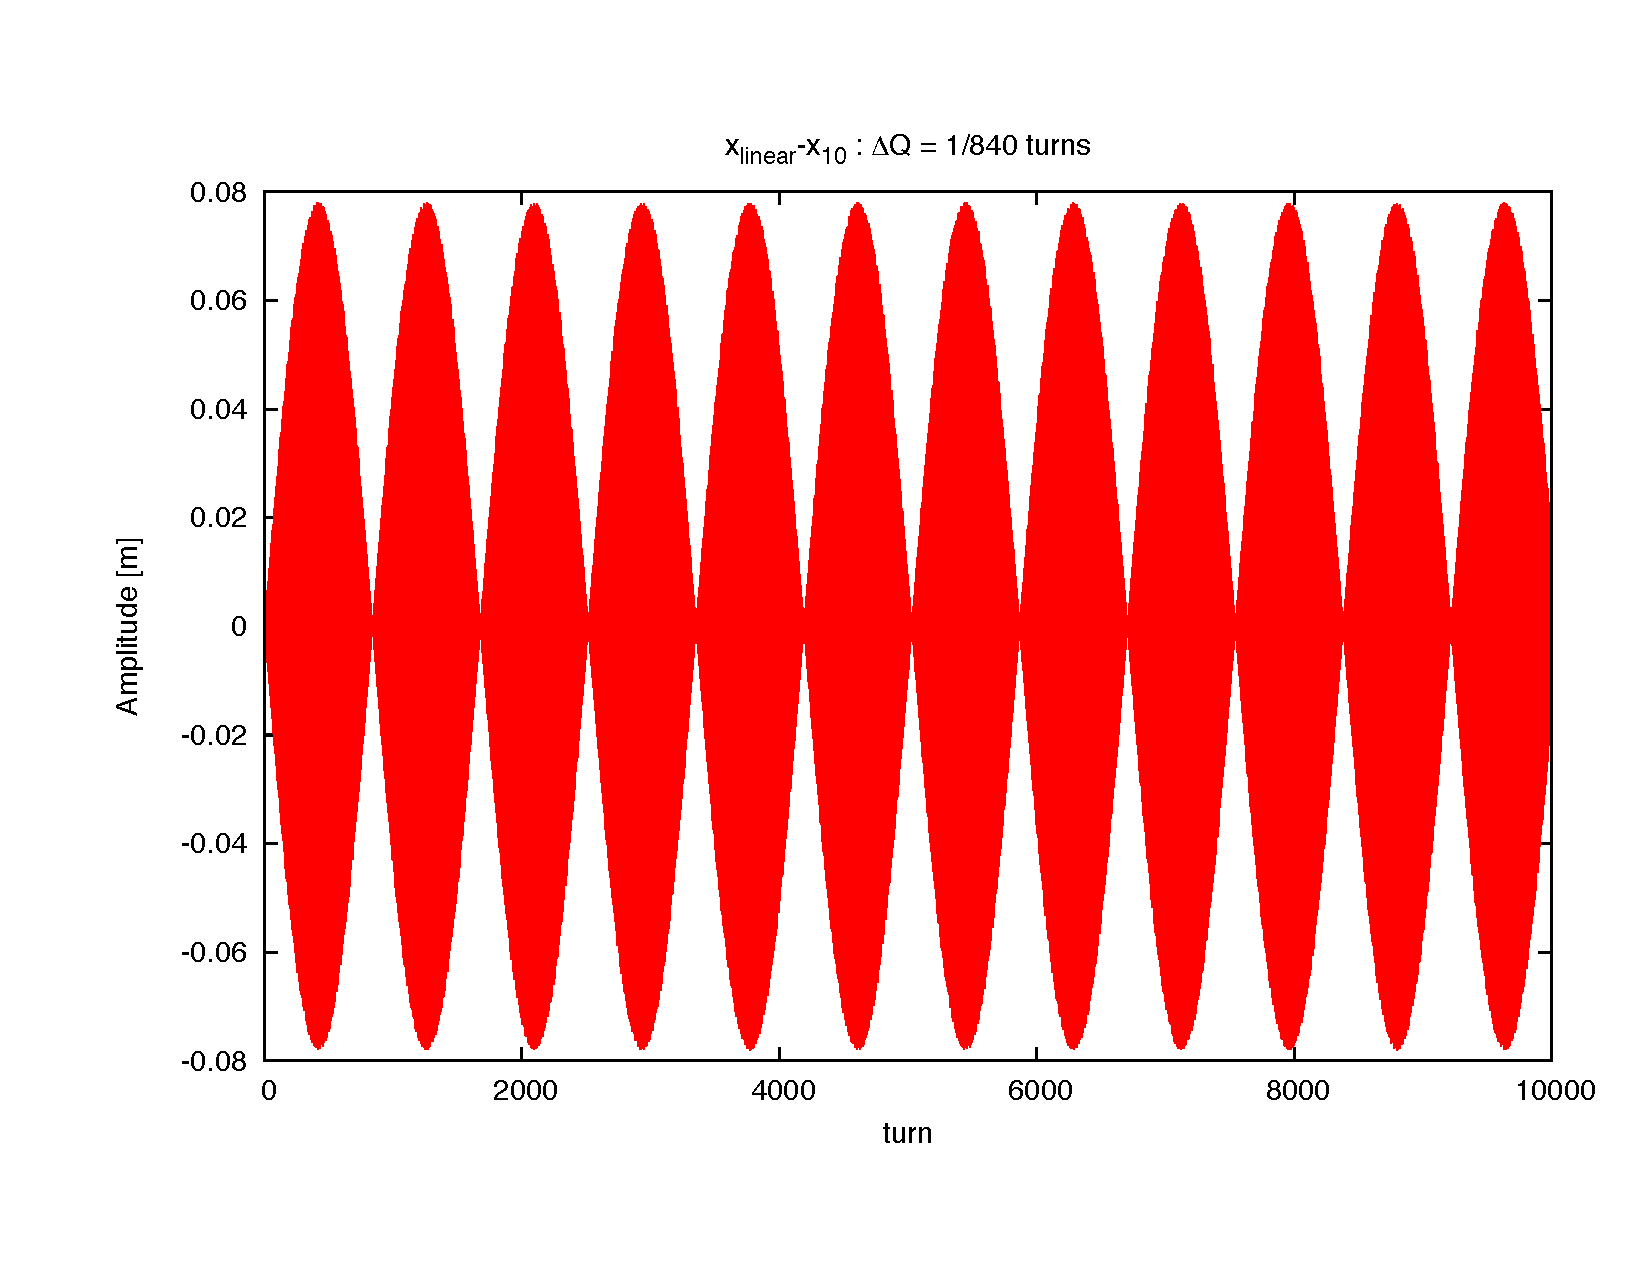
\includegraphics[trim = 0mm 0mm 0mm 0mm, clip=.false.,width=3.in]{/Users/dlr10/lepp/g-2/beamdynamics/damping_cbo/tune_difference_linear_10.pdf} 
   \caption{ stuff \label{fig:layout}}
 \end{minipage}
\hfill
\begin{minipage}[t]{0.48\textwidth}
\centering
   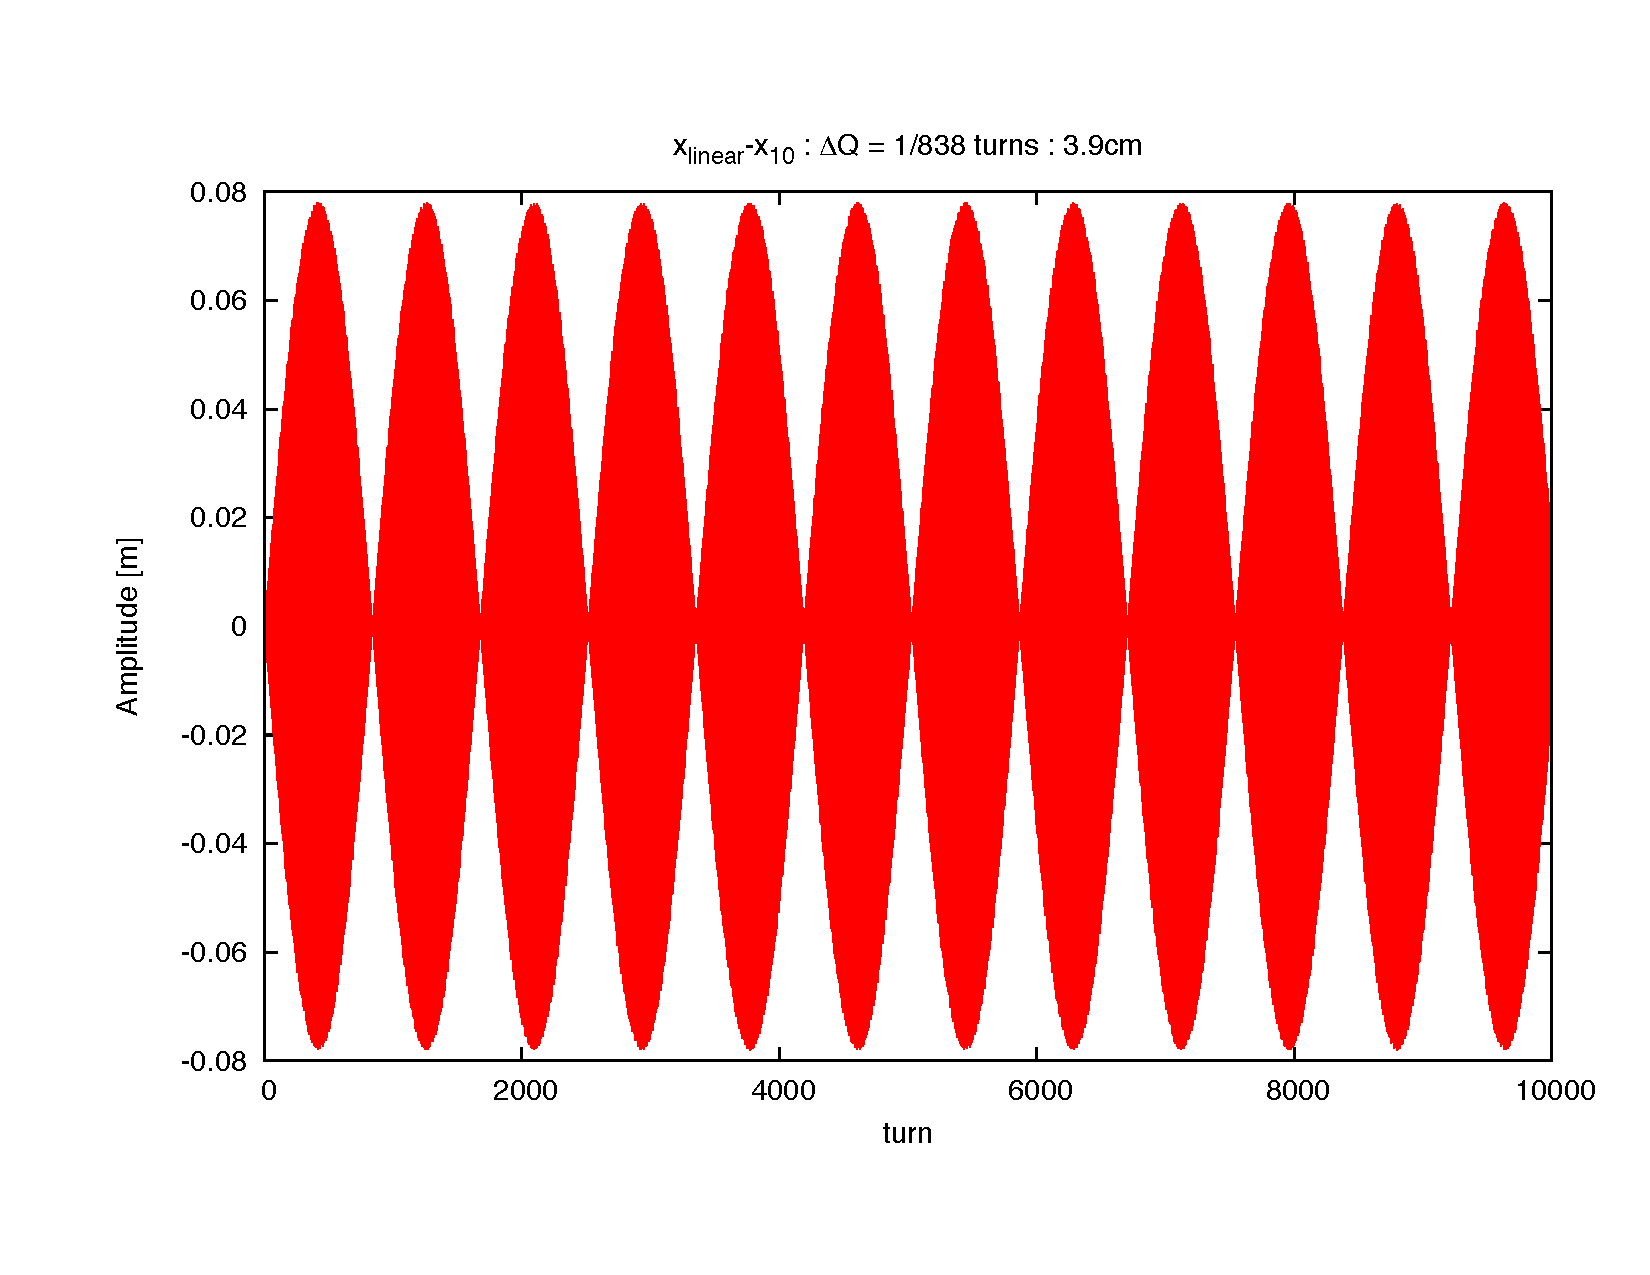
\includegraphics[trim = 0mm 0mm 0mm 0mm, clip=.false.,width=3.in]{/Users/dlr10/lepp/g-2/beamdynamics/damping_cbo/tune_difference_linear_all_39mm} 
\caption{
   \label{fig:tuneshift}}
\end{minipage}
\end{figure}

\begin{figure}[htbp] %  figure placement: here, top, bottom, or page
   \centering
   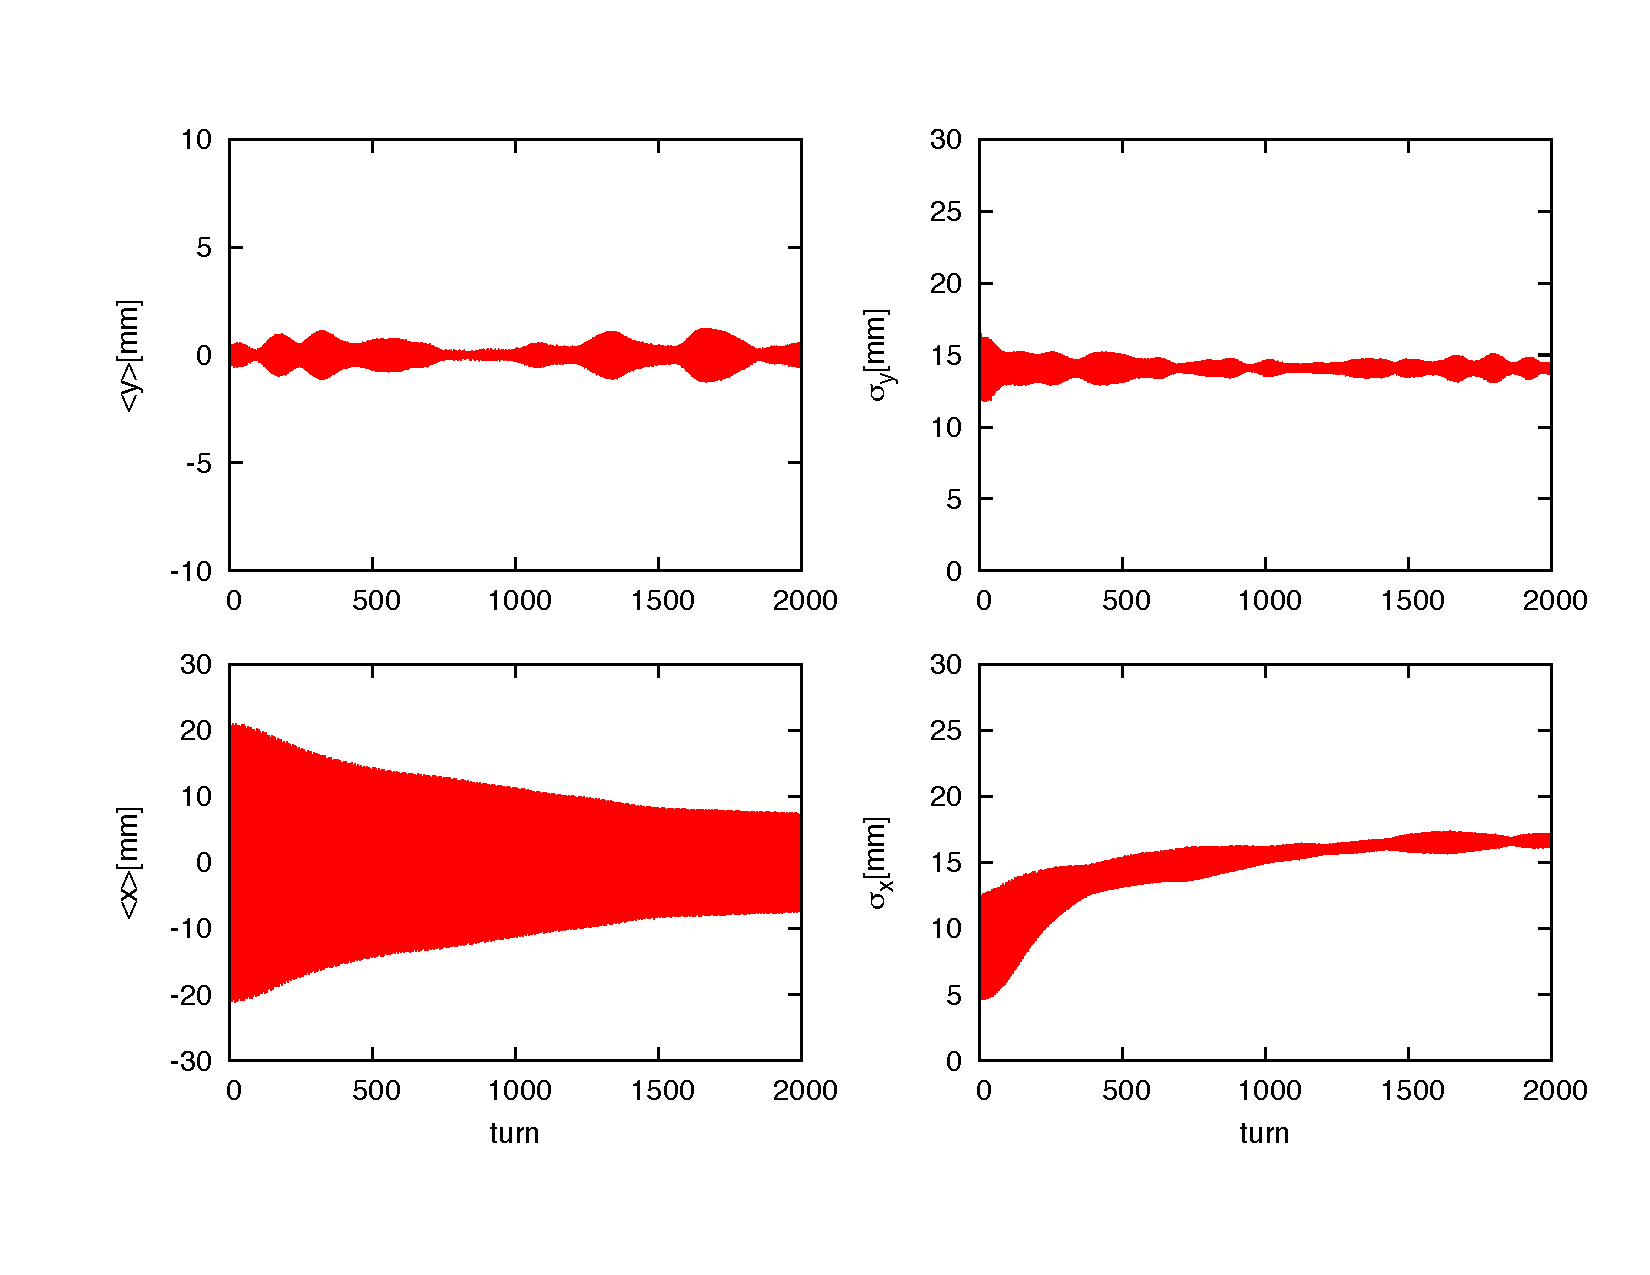
\includegraphics[trim = 40mm 0mm 0mm 0mm, clip=.false.,width=7.in]{/Users/dlr10/lepp/g-2/beamdynamics/damping_cbo/sigma_xy_20mm_qm_all_e0} 
   \caption{ stuff \label{fig:layout}}
\end{figure}

\section{Energy dependent tune}
\begin{enumerate}
\item chromaticity $Q^\prime_x= -0.14,Q^\prime_y=0.31$.
\item $\Delta E/E = \pm 0.002 \rightarrow \Delta Q = (\Delta E/E)Q_x^\prime \approx 2\cdot2.8\times 10^{-4} = 1/1785$
\item $\rightarrow$ Decoherence time due to energy spread $\approx$ 1785 turns
\end{enumerate}

\begin{figure}[htbp] %  figure placement: here, top, bottom, or page
\begin{minipage}[t]{0.48\textwidth}
   \centering
   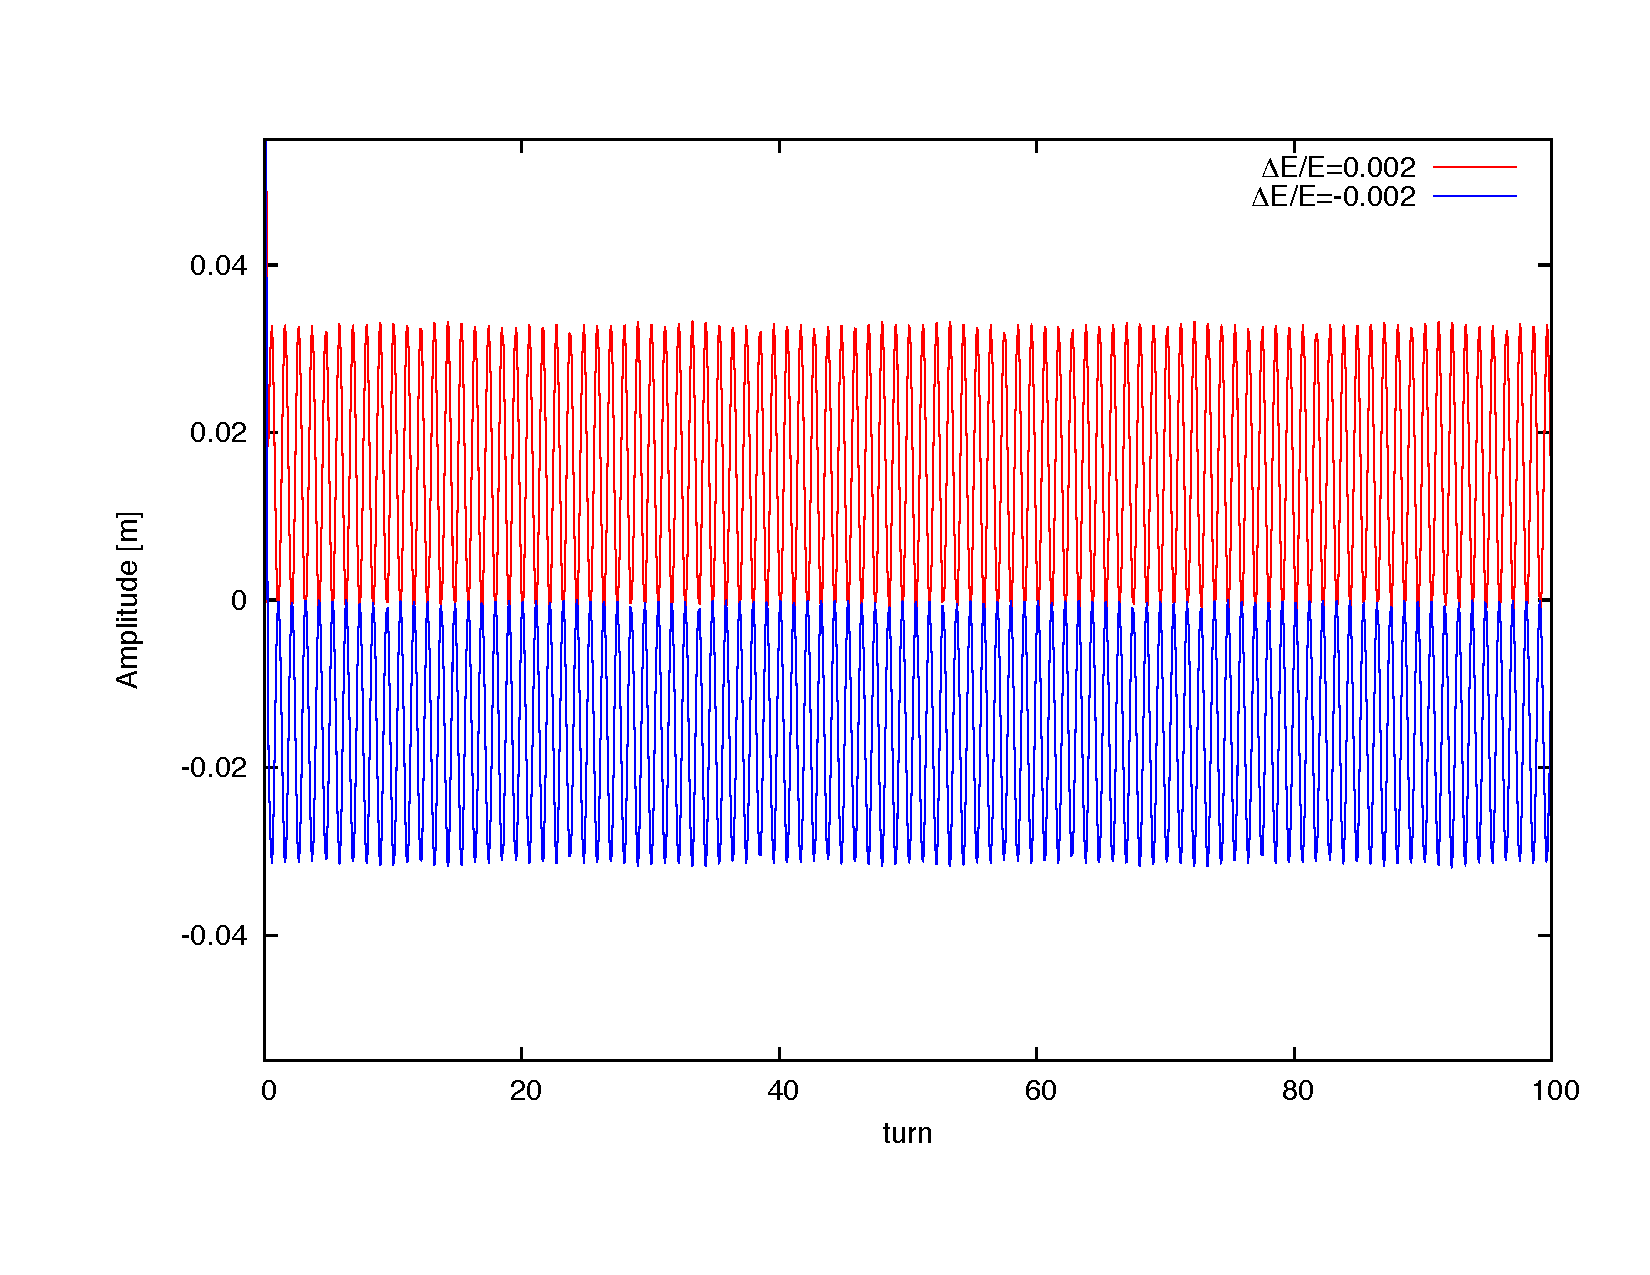
\includegraphics[trim = 0mm 0mm 0mm 0mm, clip=.false.,width=3.in]{/Users/dlr10/lepp/g-2/beamdynamics/damping_cbo/tune_overlay_denergy_002_-002.pdf} 
   \caption{ stuff \label{fig:layout}}
 \end{minipage}
\hfill
\begin{minipage}[t]{0.48\textwidth}
\centering
   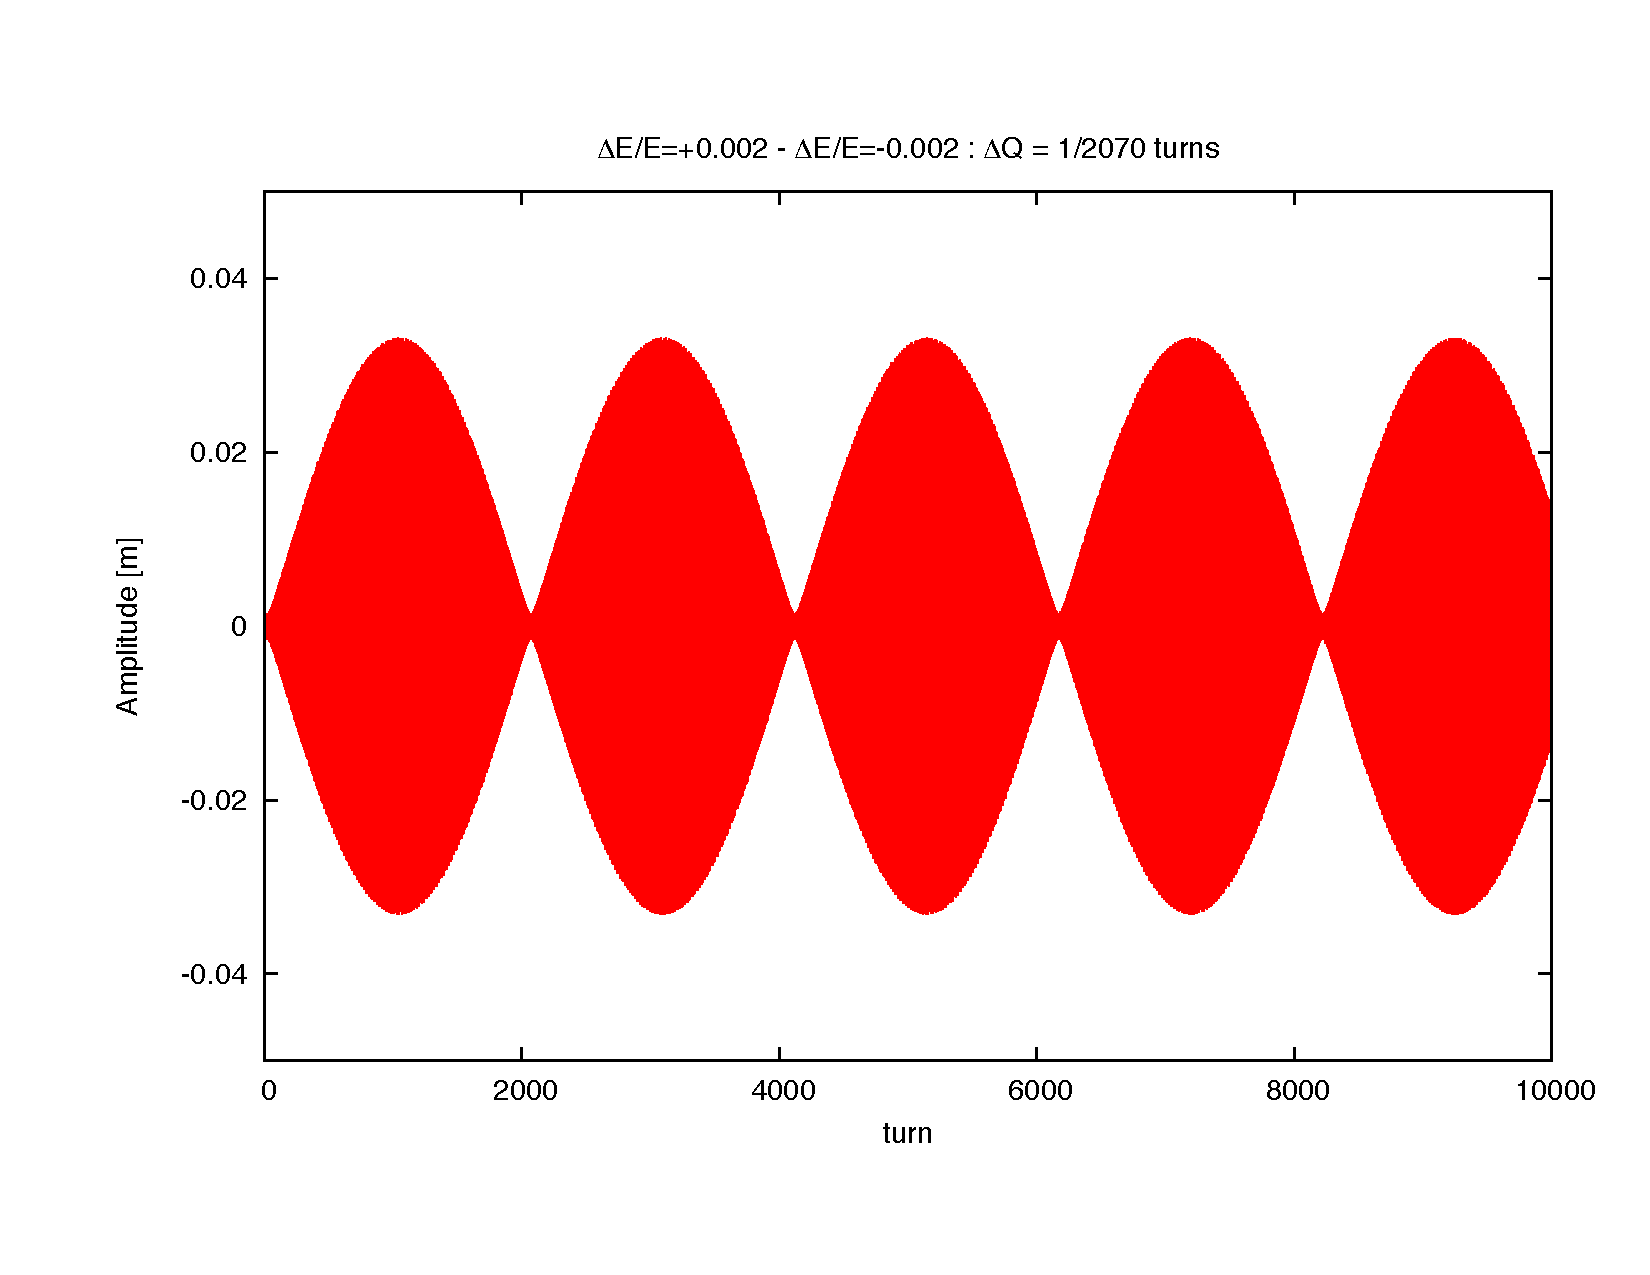
\includegraphics[trim = 0mm 0mm 0mm 0mm, clip=.false.,width=3.in]{/Users/dlr10/lepp/g-2/beamdynamics/damping_cbo/tune_difference_de002-de-002} 
\caption{
   \label{fig:tuneshift}}
\end{minipage}
\end{figure}


\begin{figure}[htbp] %  figure placement: here, top, bottom, or page
   \centering
   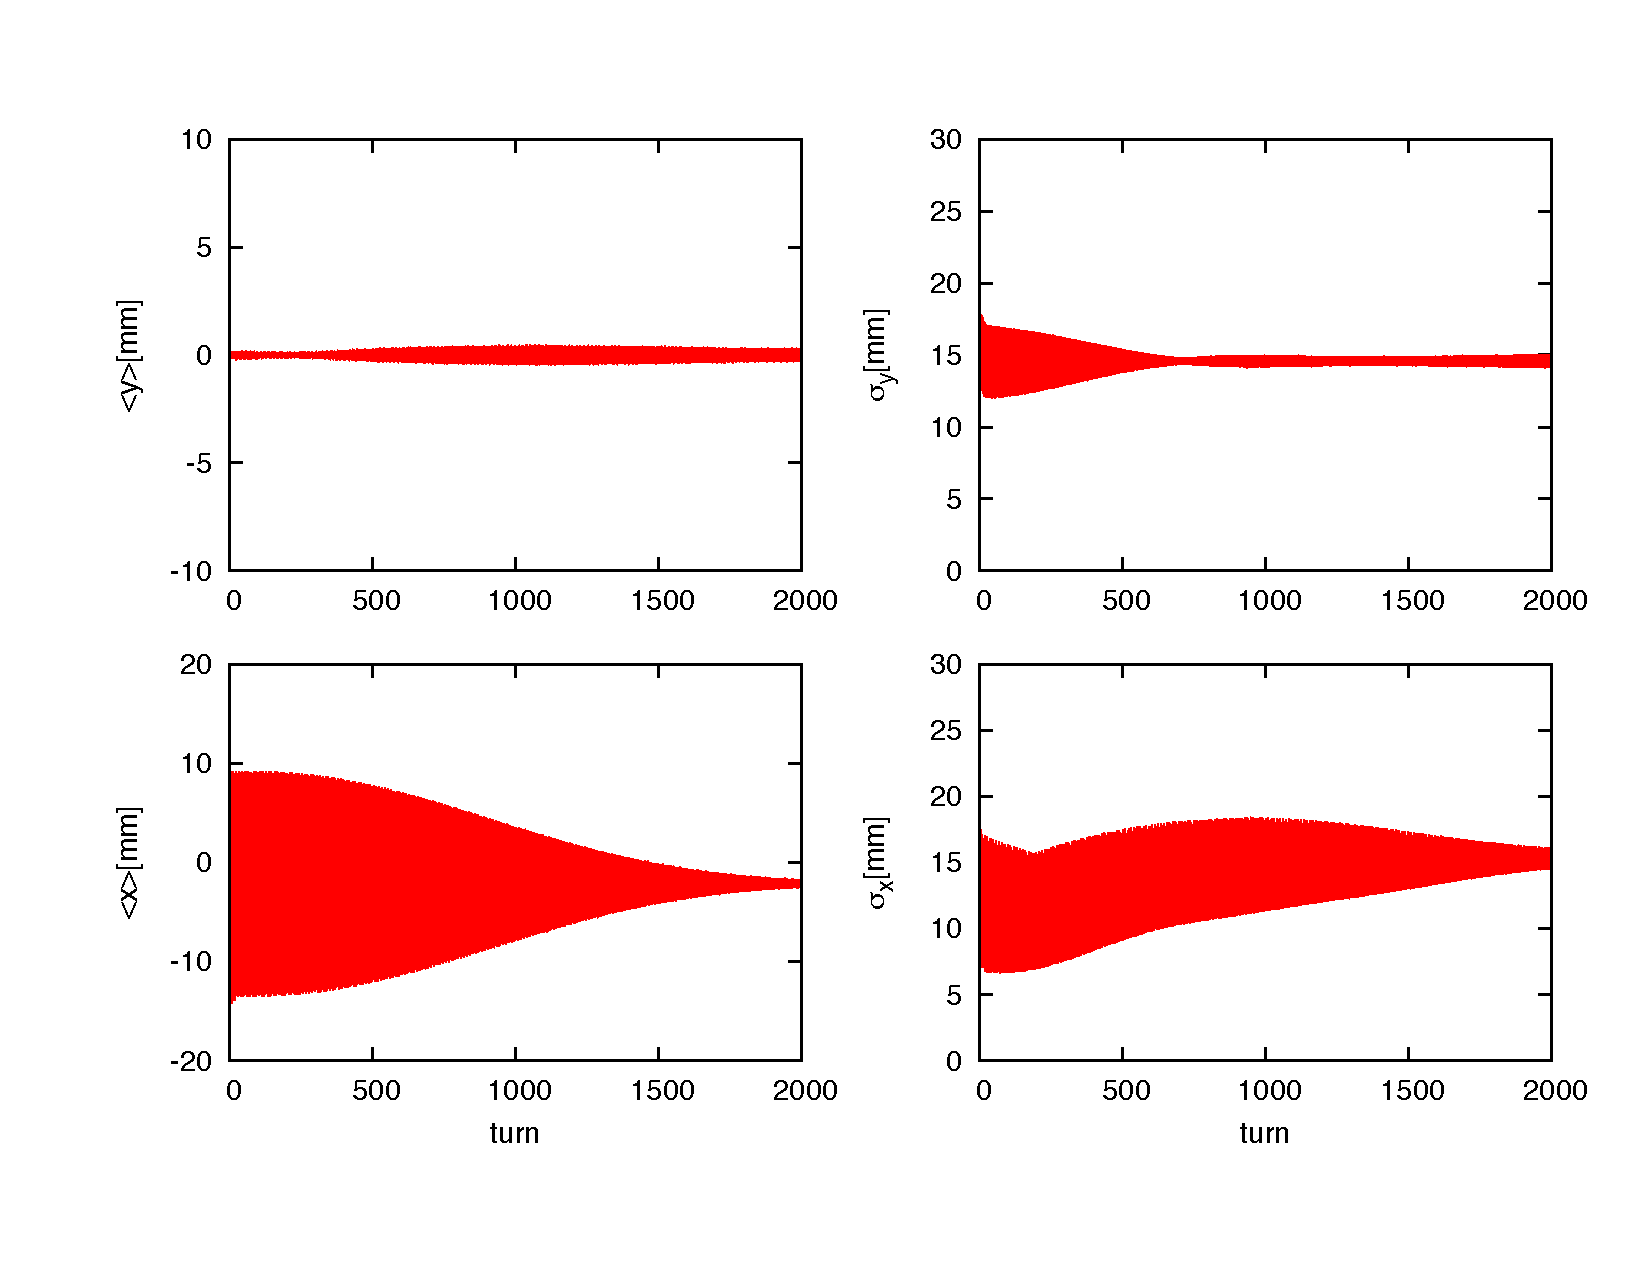
\includegraphics[trim = 40mm 0mm 0mm 0mm, clip=.false.,width=7.in]{/Users/dlr10/lepp/g-2/beamdynamics/damping_cbo/sigma_xy_qm_01_pzsig_00112} 
   \caption{ stuff \label{fig:layout}}
\end{figure}

\begin{figure}[htbp] %  figure placement: here, top, bottom, or page
   \centering
   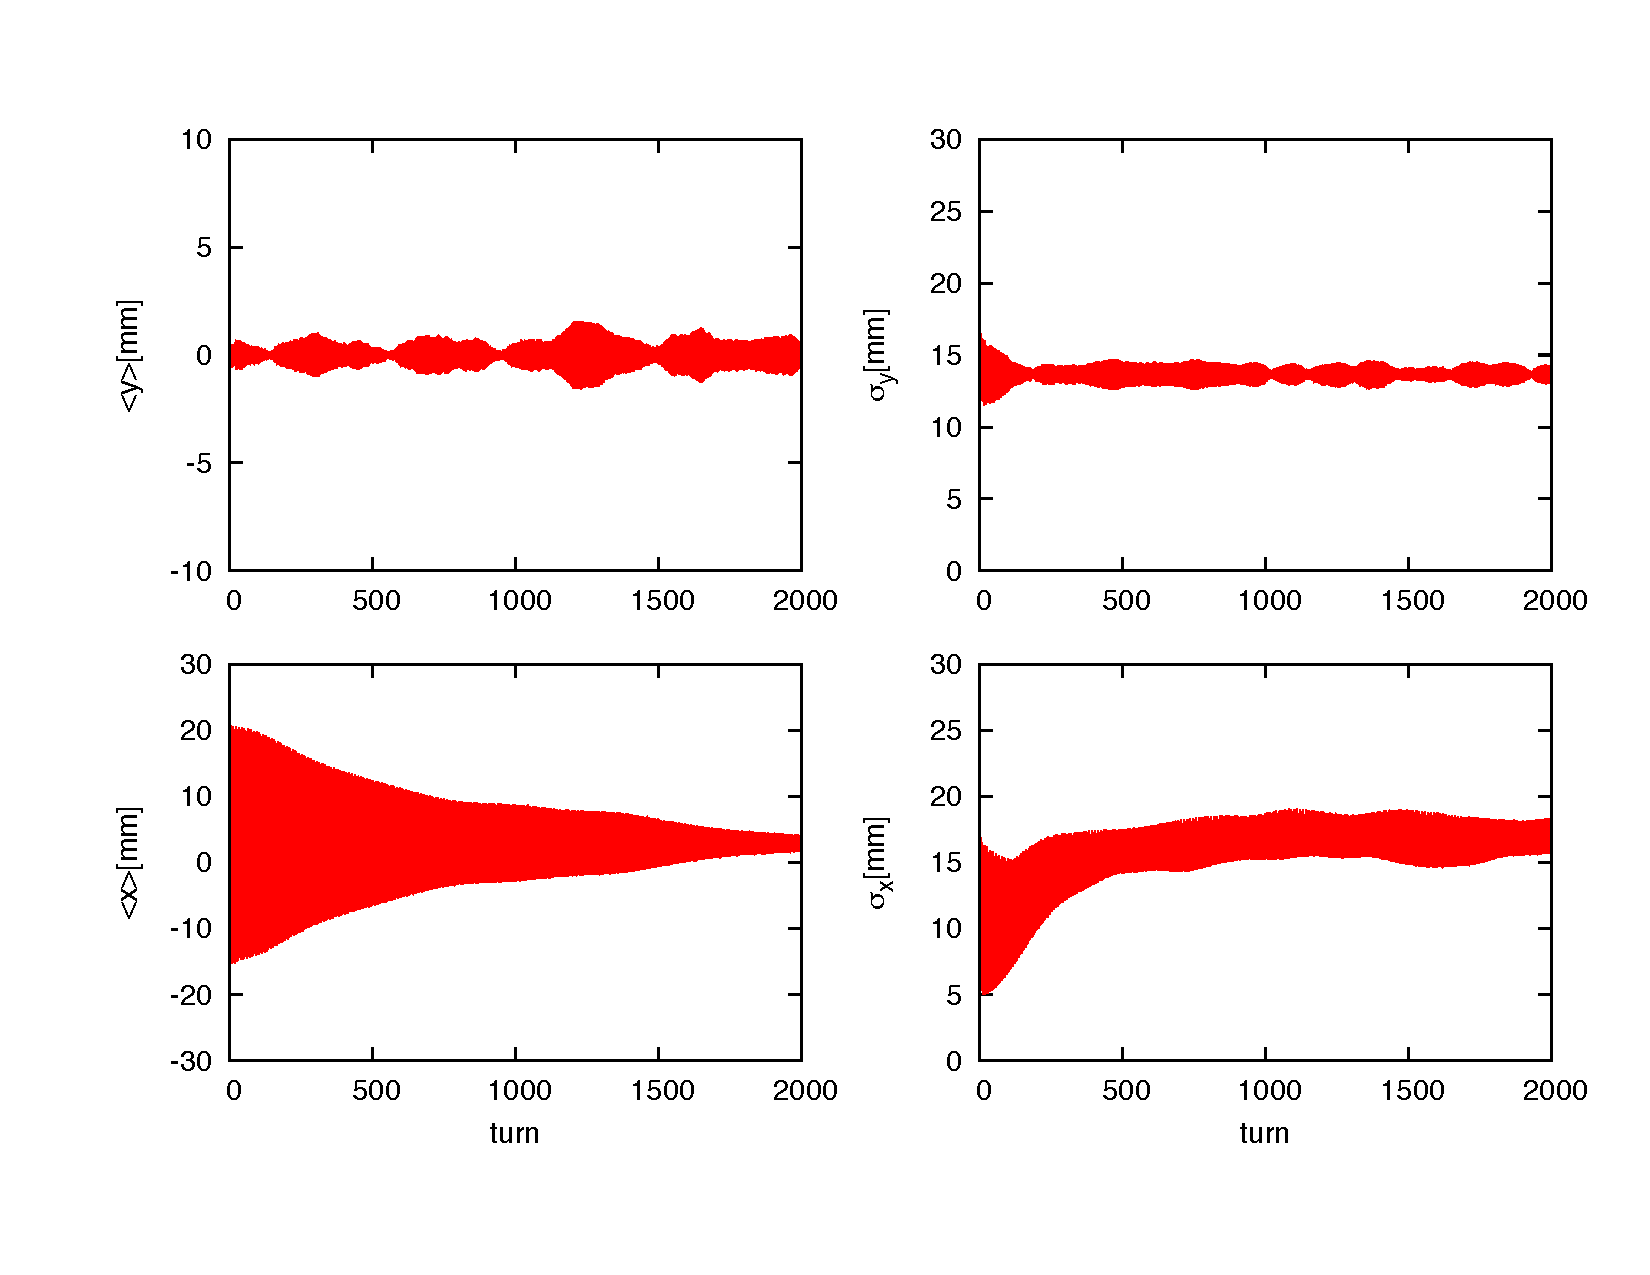
\includegraphics[trim = 40mm 0mm 0mm 0mm, clip=.false.,width=7.in]{/Users/dlr10/lepp/g-2/beamdynamics/damping_cbo/sigma_xy_mp_all_20mm_deltae00112} 
   \caption{ stuff \label{fig:layout}}
\end{figure}
\section{Conclusion}
Chromatic decoherence time ≈ 1000 turns
Amplitude dependent decoherence time (due to quad nonlinearity)  ≈ 2000 turns
   (Betatron modulation more effectively damped by amplitude dependence)
